\documentclass [12pt, a4paper, english, brazil, oneside, chapter=TITLE, section=TITLE]{abntex2}
% Para impressão use doubleside
% ---
% Arquivo com  a formatação é lido aqui. Não deve ser modificado
% ---
% ---
% Arquivo com a formatação do TCC.
% Este arquivo não deve ser modificado.
% ---
\usepackage[utf8]{inputenc}
\usepackage[T1]{fontenc}
\usepackage{amsmath}
\usepackage{amssymb,amsfonts,textcomp}
\usepackage{color}
\usepackage{array}
\usepackage{supertabular}
\usepackage{listings}         % Para as linguagens de programação
\usepackage{lastpage}		  % Usado pela Ficha catalográfica
\usepackage{indentfirst}	  % Indenta o primeiro parágrafo de cada seção.
\usepackage{hhline}
\usepackage{hyperref}
\usepackage[pdftex]{graphicx}
\graphicspath{ {./figuras/} }
\usepackage{python}
\usepackage{placeins}


% retira as mensagens de aviso do pacote Glossaries
\let\printglossary\relax
\let\theglossary\relax
\let\endtheglossary\relax
% coloca Seções em maiúsculas sem negrito no Sumário
\makeatletter
\let\oldcontentsline\contentsline
\def\contentsline#1#2{%
  \expandafter\ifx\csname l@#1\endcsname\l@section
    \expandafter\@firstoftwo
  \else
    \expandafter\@secondoftwo
  \fi
  {%
    \oldcontentsline{#1}{\normalfont\MakeTextUppercase{#2}}%
  }{%
    \oldcontentsline{#1}{#2}%
  }%
}
\makeatother
% ---
% Pacotes glossaries
% ---
\usepackage[subentrycounter,seeautonumberlist,nonumberlist=true]{glossaries}
% para usar o xindy ao invés do makeindex:
%\usepackage[xindy={language=portuguese},subentrycounter,seeautonumberlist,nonumberlist=true]{glossaries}
% ---
% Citações de referências no formato alfabético e negrito
\usepackage[alf, abnt-emphasize=bf]{abntex2cite} 
% Margens definidas em 25 mm para uso como documento em PDF
% Para imprimir use as seguintes margens:
% \usepackage[left=30mm, top=30mm, right=20 mm, bottom=20mm] {geometry}

\usepackage[margin=25 mm]{geometry}
%---
% O arquivo com o nome dos alunos e dos orientadores é lido aqui.
% Atualizar diretamente no arquivo
%---
%%%%%%%%%%%%%%%%%%%%%%%%%%%%%%%%%%%%%%%%%%%%%%%%%%%%%%%%%%%%%
% Definições de Macros utilizadas no TCC - ATUALIZE AQUI
%%%%%%%%%%%%%%%%%%%%%%%%%%%%%%%%%%%%%%%%%%%%%%%%%%%%%%%%%%%%%
\instituicao{UNIVERSIDADE FEDERAL DO RIO DE JANEIRO
\par
DEPARTAMENTO DE ENGENHARIA METALÚRGICA E DE MATERIAIS
\par
CURSO DE BACHARELADO EM ENGENHARIA METALÚRGICA}
% \title{MODELO DE MONOGRAFIA DE TRABALHO DE CONCLUSÃO DE CURSO\\ Modelo em Latex}
\title{CARACTERIZAÇÃO DA MICROESTRUTURA DE LIGAS DE ALTA ENTROPIA ATRAVÉS DE APRENDIZADO DE MÁQUINA}
\autor{Leonardo Pereira Rodrigues }
\orientador{Profa. Adriana da Cunha Rocha}
\coorientador{Profa. --}
\local{RIO DE JANEIRO, RJ - BRASIL}
\data{Junho de 2021}
\preambulo{Projeto de graduação submetido ao corpo docente do curso de engenharia metalúrgica da escola politécnica da Universidade Federal do Rio de Janeiro como parte dos requisitos necessários para a obtenção do grau de engenheiro metalúrgico.}




%%%%%%%%%%%%%%%%%%%%%%%%%%%%%%%%%%%%%%%%%%%%%%%%%%%%%%%%%%%
% Corrige a fonte dos capítulos, seções, resumos, etc.
%%%%%%%%%%%%%%%%%%%%%%%%%%%%%%%%%%%%%%%%%%%%%%%%%%%%%%%%%%%

\renewcommand{\ABNTEXchapterfont}{\bfseries \rmfamily}  % Capítulos em Bold e Maiúsculas
\renewcommand{\ABNTEXchapterfontsize}{\normalsize}
\renewcommand{\ABNTEXsectionfont}{\rmfamily}            %  Seções em  Maiúsculas apenas
\renewcommand{\ABNTEXsectionfontsize}{\normalsize}
\renewcommand{\ABNTEXsubsectionfont}{\bfseries}         % Subseções em Bold apenas
\renewcommand{\ABNTEXsubsectionfontsize}{\normalsize}
\renewcommand{\lstlistingname}{Código}                  % Nome para os códigos no texto
\renewcommand{\lstlistlistingname}{Lista de \lstlistingname s}
\makeatletter                                          % Configura a linha da lista de códigos
\renewcommand\l@lstlisting[2]{{\normalfont\@dottedtocline{1}{1.5em}{2em}{Código~#1}{#2}}}
\makeatother
\usepackage{url16023}  % para retirar < e > da URL nas referências.
%%%%%%%%%%%%%%%%%%%%%%%%%%%%%%%%%%%%%%%%%%%%%%%%%%%%%%%%%%%
% Criação de quadros com numeração
%%%%%%%%%%%%%%%%%%%%%%%%%%%%%%%%%%%%%%%%%%%%%%%%%%%%%%%%%%%
\newcommand{\quadroname}{Quadro}
\newcommand{\listofquadrosname}{Lista de quadros}

\newfloat[chapter]{quadro}{loq}{\quadroname}
\newlistof{listofquadros}{loq}{\listofquadrosname}
\newlistentry{quadro}{loq}{0}
%%%%%%%%%%%%%%%%%%%%%%%%%%%%%%%%%%%%%%%%%%%%%%%%%%%%%%%%%%%
% configurações para atender às regras da ABNT
%%%%%%%%%%%%%%%%%%%%%%%%%%%%%%%%%%%%%%%%%%%%%%%%%%%%%%%%%%%
\setfloatadjustment{quadro}{\centering}
\counterwithout{quadro}{chapter}
\renewcommand{\cftquadroname}{\quadroname\space} 
\renewcommand*{\cftquadroaftersnum}{\hfill--\hfill}
%---
% Configuração de posicionamento padrão
%---
\setfloatlocations{quadro}{hbtp}
%---
% Para ajudar nas tabelas e quadros
%---
\makeatletter
\newcommand\arraybslash{\let\\\@arraycr}
\makeatother
%%%%%%%%%%%%%%%%%%%%%%%%%%%%%%%%%%%%%%%%%%%%%%%%%%%%%%%
% Redefine a macro para imprimir a capa 
%%%%%%%%%%%%%%%%%%%%%%%%%%%%%%%%%%%%%%%%%%%%%%%%%%%%%%%
\renewcommand{\imprimircapa}{%
\begin{capa}%
\center
\imprimirinstituicao
\par
\vspace*{1cm}
\MakeUppercase{\imprimirautor}
\vfill
\begin{center}
\imprimirtitulo
\end{center}
\vfill
\imprimirlocal
\par
\imprimirdata
\vspace*{1cm}
\end{capa}
}
%%%%%%%%%%%%%%%%%%%%%%%%%%%%%%%%%%%%%%%%%%%%%%%%%%%%%%%
% Redefine a macro para imprimir a folho de rosto
%%%%%%%%%%%%%%%%%%%%%%%%%%%%%%%%%%%%%%%%%%%%%%%%%%%%%%%

\renewcommand{\imprimirfolhaderosto}{%
% \begin{figure}[b]
% \centering

\includegraphics{figuras/poli-ufrj-logo.png}
% \end{figure}
\begin{capa}%
\center
\par
\vspace*{1cm}
% \MakeUppercase{\imprimirautor}
\vfill
\begin{center}
\imprimirtitulo
\end{center}
\vfill
{\imprimirautor}
\vfill
\hspace*{\fill}\parbox[b]{.5\textwidth}{%
        \linespread{1.5}\selectfont
Projeto de graduação apresentado ao corpo docente do curso de engenharia metalúrgica da escola politécnica da Universidade Federal do Rio de Janeiro como parte dos requisitos necessários para a obtenção do grau de engenheiro metalúrgico.

}
\vfill
\flushright
Orientador: \imprimirorientador\\

% Co-orientador: \imprimircoorientador\\
\vfill
\begin{center}
\large\imprimirlocal
\par
\large\imprimirdata
\vspace*{1cm}
\end{center}
\end{capa}
}
%%%%%%%%%%%%%%%%%%%%%%%%%%%%%%%%%%%%%%%%%%%%%%%%%%%%%%%
% Informações do PDF inseridas automaticamente
% Atualizar apenas as palavras-chave se necessário
% Não modificar as cores dos links e referências
%%%%%%%%%%%%%%%%%%%%%%%%%%%%%%%%%%%%%%%%%%%%%%%%%%%%%%%
\makeatletter
\hypersetup{
pdftitle={\@title},
pdfauthor={\@author},
pdfsubject={\imprimirpreambulo},
pdfkeywords={MONOGRAFIA}{CIÊNCIA DA COMPUTAÇÃO}{DCC-UFRJ},
pdfcreator={LaTeX with abnTeX2},
colorlinks=true,
linkcolor=black,
citecolor=black,
urlcolor=black
}
\makeatother
%%%%%%%%%%%%%%%%%%%%%%%%%%%%%%%%%%%%%%%%%%%%%%%%%%%%
% Definição das Linguagens de Programação
%%%%%%%%%%%%%%%%%%%%%%%%%%%%%%%%%%%%%%%%%%%%%%%%%%%%
\definecolor{dkgreen}{rgb}{0,0.6,0}
\definecolor{gray}{rgb}{0.5,0.5,0.5}
\definecolor{purple}{rgb}{0.8,0,0.3}
\definecolor{orange}{rgb}{1,0.4,0}
\definecolor{lightlightgray}{rgb}{.95,.95,.95}
\definecolor{lightgray}{rgb}{.9,.9,.9}
\definecolor{lightgray2}{rgb}{.85,.85,.85}
\definecolor{darkgray}{rgb}{.4,.4,.4}
%---
% Comando para inserir a listagem de código, tem 4 parâmetros
% Linguagem, Caption, Label, Nome do Arquivo
%---
\newcommand{\includecode}[4][C]{\mbox{\lstinputlisting[caption=#2, label=#3, escapechar=, style=custom#1]{#4}}}

%---
%Define características em comum e numeração sequencial 
%---
\lstset{numberbychapter=false,framexleftmargin=5mm,  frame=shadowbox, rulesepcolor=\color{gray}}
%---
% A leitura da formatação das linguagens é feita aqui. 
% Modifique diretamente no arquivo.
%
%%%%%%%%%%%%%%%%%%%%%%%%%%%%%%%%%%%%%%%%%%%%%%%%%%%%
% Aqui você pode personalizar a linguagem C  
%%%%%%%%%%%%%%%%%%%%%%%%%%%%%%%%%%%%%%%%%%%%%%%%%%%%
\lstdefinestyle{customC}{
      language = C,
      breaklines=true,
      basicstyle=\footnotesize\ttfamily,
      keywordstyle=\bfseries\color{blue},
      commentstyle=\itshape\color{purple},
      identifierstyle=\color{black},
      stringstyle=\color{orange},
      showstringspaces=false}

% \includecode[Java]{Exemplo em Linguagem Java} {alg:codigo2}{codigos/codigo.java}

%%%%%%%%%%%%%%%%%%%%%%%%%%%%%%%%%%%%%%%%%%%%%%%%%%%%
% Aqui você pode personalizar a linguagem Java 
%%%%%%%%%%%%%%%%%%%%%%%%%%%%%%%%%%%%%%%%%%%%%%%%%%%%       
\lstdefinestyle{customJava}{
      language = Java,
      breaklines=true,
      basicstyle=\footnotesize\ttfamily,
      keywordstyle=\bfseries\color{blue},
      commentstyle=\itshape\color{purple},
      identifierstyle=\color{black},
      stringstyle=\color{orange},
      showstringspaces=false}
%%%%%%%%%%%%%%%%%%%%%%%%%%%%%%%%%%%%%%%%%%%%%%%%%%%%
% Aqui você pode personalizar a linguagem C++
%%%%%%%%%%%%%%%%%%%%%%%%%%%%%%%%%%%%%%%%%%%%%%%%%%%%  
\lstdefinestyle{customC++}{
      language = C++,
      breaklines=true,
      basicstyle=\footnotesize\ttfamily,
      keywordstyle=\bfseries\color{blue},
      commentstyle=\itshape\color{purple},
      identifierstyle=\color{black},
      stringstyle=\color{orange},
      showstringspaces=false}
%%%%%%%%%%%%%%%%%%%%%%%%%%%%%%%%%%%%%%%%%%%%%%%%%%%%
% Aqui você pode personalizar a linguagem Javascript
%%%%%%%%%%%%%%%%%%%%%%%%%%%%%%%%%%%%%%%%%%%%%%%%%%%%        
\lstdefinestyle{customJavaScript}{
      language = JavaScript,
      breaklines=true,
      basicstyle=\footnotesize\ttfamily,
      keywordstyle=\bfseries\color{blue},
      commentstyle=\itshape\color{purple},
      identifierstyle=\color{black},
      stringstyle=\color{orange},
      showstringspaces=false}
      
% Javascript
\lstdefinelanguage{JavaScript}{
    aboveskip=15pt,
    keywords={typeof, new, true, false, catch, function, return, null, catch, switch, var, if, in, while, do, else, case, break},
    keywordstyle=\color{blue}\bfseries,
    ndkeywords={class, export, boolean, throw, implements, import, this},
    ndkeywordstyle=\color{darkgray}\bfseries,
    identifierstyle=\color{black},
    sensitive=false,
    comment=[l]{//},
    morecomment=[s]{/*}{*/},
    commentstyle=\color{purple}\ttfamily,
    stringstyle=\color{red}\ttfamily,
    morestring=[b]',
    morestring=[b]",
    rulecolor=\color{lightgray2},
    breaklines=true,
    basicstyle=\footnotesize\ttfamily,
    frame=single,
    backgroundcolor=\color{lightlightgray}
}
%%%%%%%%%%%%%%%%%%%%%%%%%%%%%%%%%%%%%%%%%%%%%%%%%%%%
% Aqui você pode personalizar o formato JSON
%%%%%%%%%%%%%%%%%%%%%%%%%%%%%%%%%%%%%%%%%%%%%%%%%%%%        
\lstdefinestyle{customJSON}{
      language = JSON,
      breaklines=true,
      basicstyle=\footnotesize\ttfamily,
      keywordstyle=\bfseries\color{blue},
      commentstyle=\itshape\color{purple},
      identifierstyle=\color{black},
      stringstyle=\color{orange},
      showstringspaces=false}
      
% JSON
\lstdefinelanguage{JSON}{
    aboveskip=15pt,
    string=[s]{"}{"},
    stringstyle=\color{blue},
    comment=[l]{:},
    commentstyle=\color{black},
    rulecolor=\color{lightgray2},
    breaklines=true,
    basicstyle=\footnotesize\ttfamily,
    frame=single,
    backgroundcolor=\color{lightlightgray}
}
%%%%%%%%%%%%%%%%%%%%%%%%%%%%%%%%%%%%%%%%%%%%%%%%%%%%
% Aqui você pode personalizar a linguagem de montagem do SAPIENS
%%%%%%%%%%%%%%%%%%%%%%%%%%%%%%%%%%%%%%%%%%%%%%%%%%%%       
\lstdefinestyle{customSapiens}{
      language = Sapiens,
      breaklines=true,
      basicstyle=\footnotesize\ttfamily,
      keywordstyle=\bfseries\color{blue},
      commentstyle=\itshape\color{purple},
      identifierstyle=\color{black},
      stringstyle=\color{orange},
      showstringspaces=false}

% Linguagem de Montagem    
\lstdefinelanguage{Sapiens}{
    aboveskip=15pt,
    keywordstyle=\color{blue}\bfseries,
    comment=[l]{;},
    commentstyle=\color{purple},
    rulecolor=\color{lightgray2},
    breaklines=true,
    basicstyle=\footnotesize\ttfamily,
    frame=single,
    backgroundcolor=\color{lightlightgray},
    language=[x86masm]Assembler,
    morekeywords={DB, DS, DW, JN, JSR, LDA, ORG, STA, STS, TRAP}
}

%%%%%%%%%%%%%%%%%%%%%%%%%%%%%%%%%%%%%%%%%%%%%%%%%%%%
% Aqui você pode personalizar a linguagem Python 
%%%%%%%%%%%%%%%%%%%%%%%%%%%%%%%%%%%%%%%%%%%%%%%%%%%%       
\lstdefinestyle{customPython}{
      language = Python,
      breaklines=true,
      basicstyle=\footnotesize\ttfamily,
      keywordstyle=\bfseries\color{blue},
      commentstyle=\itshape\color{darkgray},
      identifierstyle=\color{black},
      stringstyle=\color{orange},
      showstringspaces=true}

      
      
% \lstset{language=Python, 
%         basicstyle=\ttfamily\small, 
%         keywordstyle=\color{keywords},
%         commentstyle=\color{comments},
%         stringstyle=\color{red},
%         showstringspaces=false,
%         identifierstyle=\color{green},
%         procnamekeys={def,class}}


%---
% FIM
%---

%=====================================================================
% Definição do conteúdo de "dedicatória"
%=====================================================================
\newcommand{\makededicationpage}{

    \vspace*{\fill}

  \hspace*{\fill}\parbox[b]{.5\textwidth}{%
  \begin{flushright}
\begin{dedicatoria}
\vspace*{\fill}
Dedico aos meus pais Eduardo e Sueli, e a todos que me deram força esperança de continuar até o fim.
\vspace*{\fill}
\end{dedicatoria}
\end{flushright}
  }
  
  
  \pagebreak
}{}

%=====================================================================
% ---
% GLOSSÁRIO
% ---
\makeglossaries
% ---
% Entradas do glossário
% ---
\newglossaryentry{componente}{
               name={componente},
               plural={componentes},
%               parent=pai,
               description={descrição da entrada componente} }
 
\newglossaryentry{equilibrio}{
                name={equilíbrio da configuração},
                see=[veja também]{componente},
                description={consistência entre os \glspl{componente}}
                }

\newglossaryentry{latex}{
                name={LaTeX},
                description={ferramenta de computador para autoria de documentos criada por D. E. Knuth} }

\newglossaryentry{abntex2}{
                name={abnTeX2},
                see=latex,
                description={suíte para LaTeX que atende os requisitos das
                normas da ABNT para elaboração de documentos técnicos e científicos brasileiros} }
                
\newglossaryentry{maths}
{
    name=matemática,
    description={Matemática é o que os matemáticos fazem}
}

\newglossaryentry{formula}
{
        name=formula,
        description={Uma expressão matemática}
}
 
\newacronym{mdc}{MDC}{Maior Divisor Comum}
 
\newacronym{mmc}{MMC}{Mínimo Múltipo Comum}


% ---
%\item [Palavra] Significado da palavra

%\item [Palavra 2] Significado da palavra 2
% ---
%%%%%%%%%%%%%%%%%%%%%%%%%%%%%%%%%%%%%%%%%%%%%%%%%%%%%%%%%%%%
% I N I C I O  D O  D O C U M E N T O
%%%%%%%%%%%%%%%%%%%%%%%%%%%%%%%%%%%%%%%%%%%%%%%%%%%%%%%%%%%%
\begin{document}
\pretextual

%%%%%%%%%%%%%%%%%%%%%%%%%%%%%%%%%%%%%%%%%%%%%%%%%%%%%%%%%%%%
% C A P A (OBRIGATÓRIO)
%%%%%%%%%%%%%%%%%%%%%%%%%%%%%%%%%%%%%%%%%%%%%%%%%%%%%%%%%%%%

\setcounter{page}{1}
% \imprimircapa

%%%%%%%%%%%%%%%%%%%%%%%%%%%%%%%%%%%%%%%%%%%%%%%%%%%%%%%%%%%%
% F O L H A  D E  R O S T O  (OBRIGATÓRIO)
%%%%%%%%%%%%%%%%%%%%%%%%%%%%%%%%%%%%%%%%%%%%%%%%%%%%%%%%%%%%

\imprimirfolhaderosto

%%%%%%%%%%%%%%%%%%%%%%%%%%%%%%%%%%%%%%%%%%%%%%%%%%%%%%%%%
% F O L H A   D E   A P R O V A Ç Ã O  (OBRIGATÓRIO)
%%%%%%%%%%%%%%%%%%%%%%%%%%%%%%%%%%%%%%%%%%%%%%%%%%%%%%%%%
% Isto é um exemplo folha de aprovação.
% Substitua todo o conteúdo desta página por uma
% imagem da página assinada pela banca com o comando abaixo:
% \includepdf{folhadeaprovacao_final.pdf}
%%%%%%%%%%%%%%%%%%%%%%%%%%%%%%%%%%%%%%%%%%%%%%%%%%%%%%%%%

\begin{folhadeaprovacao}
\vspace*{\fill}
\begin{center}
     
    
    \begin{center}
      \imprimirtitulo \\
    \end{center}
    \vspace*{\fill}
    {\imprimirautor}
    \vspace*{\fill}
  \end{center}
  
   \MakeUppercase{\noindent{\imprimirpreambulo}} 


\vspace*{\fill}
    \begin{flushleft}
 % Alterar a data ou preencher à mão
%   Aprovado em \_\_\_ de \_\_\_\_\_\_\_\_\_\_\_\_\_\_ de \_\_\_\_\_\_\_
  \par
  \vspace*{\fill}

EXAMINADO POR:
\end{flushleft}


  \hspace*{\fill}\parbox[b]{.5\textwidth}{%
  \begin{flushright}
  
   \assinatura{Profa. Adriana da Cunha Rocha \\ Orientadora}
%   \vspace*{\onelineskip}
   \assinatura{Nome do Professor1 \\ Titulação (Instituição)}
%   \vspace*{\onelineskip}
   \assinatura{Nome do Professor2\\ Titulação (Instituição)}
   %\assinatura{Nome do Professor, Titulação (Instituição)}
   %\assinatura{Nome do Professor, Titulação (Instituição)}
\vspace*{\fill}
\vspace*{\fill}

\end{flushright}
  }
  \vspace*{\fill}
 \begin{center}
\large\imprimirlocal
\par
\large\imprimirdata
% \vspace*{1cm}
\end{center}


\end{folhadeaprovacao}


%%%%%%%%%%%%%%%%%%%%%%%%%%%%%%%%%%%%%%%%%%%%%%%%%%%%%%%%%%%%
% F I C H A   C A T A L O G R Á F I A  (OBRIGATÓRIO)
%%%%%%%%%%%%%%%%%%%%%%%%%%%%%%%%%%%%%%%%%%%%%%%%%%%%%%%%%%%%
% Ficha catalográfica (obrigatório)
% Para elaborar a ficha catalográfica siga as instruções em
% http://fichacatalografica.sibi.ufrj.br/}
%%%%%%%%%%%%%%%%%%%%%%%%%%%%%%%%%%%%%%%%%%%%%%%%%%%%%%%%%%%%
\pagestyle{plain}
\pagenumbering{roman}
\aliaspagestyle{chapter}{plain}
% \aliaspagestyle{graphics}{plain}



\vspace*{1cm}
\begin{fichacatalografica}
\begin{figure}[b]
\centering
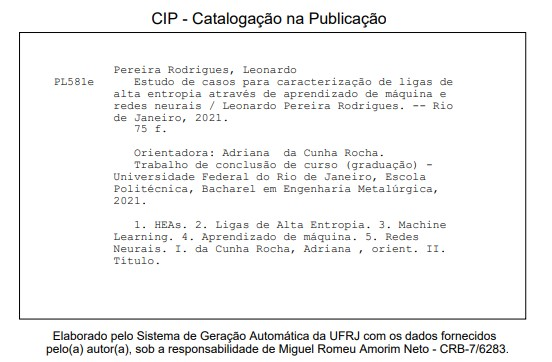
\includegraphics[width=14.217cm,height=9.929cm]{CIP_colacao.jpg}
% 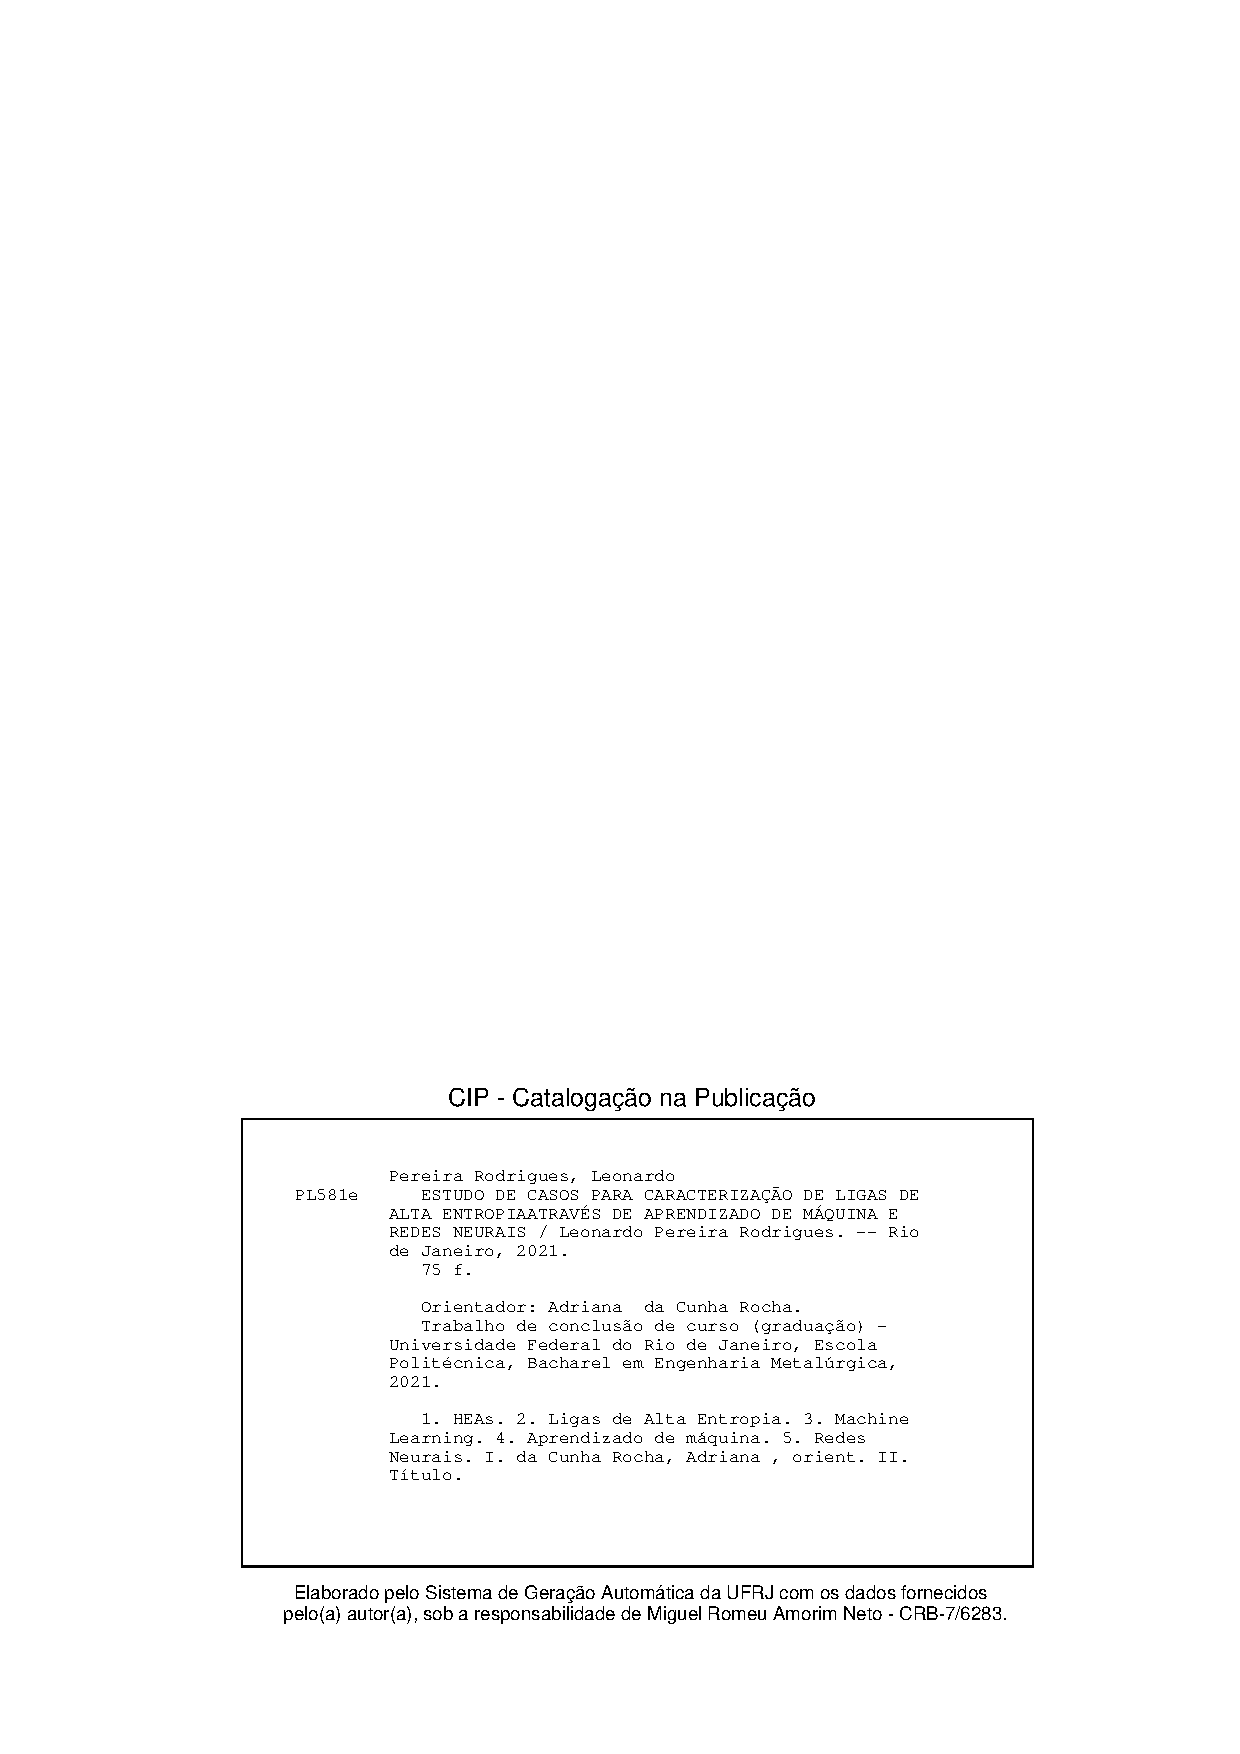
\includepdf{file.pdf}
\end{figure}
% Opcionalmente você pode usar

\end{fichacatalografica}
\pagebreak


%%%%%%%%%%%%%%%%%%%%%%%%%%%%%%%%%%%%%%%%%%%%%%%%%%%%%%%%%%%
% D E D I C A T O R I A  (OPCIONAL)
%%%%%%%%%%%%%%%%%%%%%%%%%%%%%%%%%%%%%%%%%%%%%%%%%%%%%%%%%%%

% \begin{dedicatoria}
\vspace*{\fill}
Dedico aos meus pais Eduardo e Sueli, e a todos que me deram força esperança de continuar até o fim.
\vspace*{\fill}
\end{dedicatoria}
\makededicationpage

%%%%%%%%%%%%%%%%%%%%%%%%%%%%%%%%%%%%%%%%%%%%%%%%%%%%%%%%%%%%
% A G R A D E C I M E N T O S  (OPCIONAL)
%%%%%%%%%%%%%%%%%%%%%%%%%%%%%%%%%%%%%%%%%%%%%%%%%%%%%%%%%%%% 

\begin{agradecimentos}

Quero agradecer, primeiramente, a Deus, pelo fôlego de vida para superar todos os desafios dessa jornada.

Agradeço também aos meus pais Eduardo e Sueli e ao meu irmão Vitor, por estarem ao meu lado em todos os momentos da minha vida orando por mim, me dando apoio e força.

Ao Igor Cândido, que sem ele seria quase impossível passar pelas dificuldades das disciplinas do departamento. Aos meus POWER amigos Adriano Caldeira,  Bernardo Magaldi, Henrique Dias, Jair Braga, João Pontes, Júlio Franco,  Kawan Bartras, Marcus Pessanha, Mathias Gregório, Guilherme. 

Um agradecimento especial ao Glauber Rosário e a família dele por terem me acolhido durante meu estágio de verão no Espírito Santo.

À irmandade do "sabrino": Pedro Leitão, Rodrigo Gimenes, Paulo Cysne, Daniel, por todas as reuniões de estudos, resumos, exercícios feitos juntos que aconteceram. 

A todos do bloco F e arredores, especialmente ao Cesar da Xerox, ao Betão da EQ.


\end{agradecimentos}

%%%%%%%%%%%%%%%%%%%%%%%%%%%%%%%%%%%%%%%%%%%%%%%%%%%%%%%%%%%%
% E P I G R A F E (OPCIONAL E SEM TÍTULO)
%%%%%%%%%%%%%%%%%%%%%%%%%%%%%%%%%%%%%%%%%%%%%%%%%%%%%%%%%%%% 

\begin{epigrafe}
\vspace*{\fill}
\begin{flushright}
Epígrafe: É um item onde o autor apresenta a citação de um texto que seja relacionado com o tema do trabalho, seguido da indicação de autoria do mesmo.\\
(texto iniciando do meio da página alinhado à direita)\\
\vspace{\onelineskip}
\textit{‘‘Few are those who see with their \\
own eyes and feel with their own hearts."\\}
\vspace{\onelineskip}
{\bfseries
Albert Einstein 
\par}
(Nome do autor da epígrafe)
\end{flushright}
\end{epigrafe}


%%%%%%%%%%%%%%%%%%%%%%%%%%%%%%%%%%%%%%%%%%%%%%%%%%%%%%%%%%%%
% R E S U M O    E M    P O R T U G U Ê S  (OBRIGATÓRIO)
%%%%%%%%%%%%%%%%%%%%%%%%%%%%%%%%%%%%%%%%%%%%%%%%%%%%%%%%%%%%

\begin{resumo}
\begin{SingleSpace}
Resumo em português. O texto deve ser digitado ou datilografado em um só parágrafo com \textbf{espaçamento simples} e conter de \textbf{150 a 500} palavras. Utilizar a terceira pessoa do singular, os verbos na voz ativa e evitar o uso de símbolos e contrações que não sejam de uso corrente. O resumo deve ressaltar o  objetivo, o método, os resultados e as conclusões do documento. As palavras-chave devem figurar logo abaixo do resumo, antecedidas da expressão \textbf{Palavras-chave:}, separadas entre si por
 ponto e finalizadas também por ponto.
\end{SingleSpace}
\vspace{\onelineskip}
\textbf{Palavras-chave}: latex. abntex. editoração de texto.

\end{resumo}

% Palavras-chave separadas e finalizadas por ponto




%%%%%%%%%%%%%%%%%%%%%%%%%%%%%%%%%%%%%%%%%%%%%%%%%%%%%%%%%%%%
% A B S T R A C T  (MANDATORY)
%%%%%%%%%%%%%%%%%%%%%%%%%%%%%%%%%%%%%%%%%%%%%%%%%%%%%%%%%%%%

\begin{resumo}[Abstract]
\begin{otherlanguage*}{english}
\begin{SingleSpace}
Abstract in english. The text should be typed or typed in a single paragraph with \textbf{single spacing} and contain between 150 and 500 words. Use the third person singular, the verbs in the active voice and avoid the use of symbols and contractions that are not of
current use.
\end{SingleSpace}

%Eventually you can also write it in spanish \textit{(resumen}), french \textit{(résumé)}, italian \textit{(riassunto)} etc.

\vspace{\onelineskip}
   \textbf{Keywords}: latex. abntex. text editoration.
 \end{otherlanguage*}
\end{resumo}




  


%%%%%%%%%%%%%%%%%%%%%%%%%%%%%%%%%%%%%%%%%%%%%%%%%%%%%%%%%%%%
% L I S T A   D E   I L U S T R A Ç Õ E S  (OPCIONAL)
%%%%%%%%%%%%%%%%%%%%%%%%%%%%%%%%%%%%%%%%%%%%%%%%%%%%%%%%%%%%

\pdfbookmark[0]{\listfigurename}{lof}
\listoffigures*
\cleardoublepage

%%%%%%%%%%%%%%%%%%%%%%%%%%%%%%%%%%%%%%%%%%%%%%%%%%%%%%%%%%%%
% L I S T A   D E   C Ó D I G O S (OPCIONAL)
%%%%%%%%%%%%%%%%%%%%%%%%%%%%%%%%%%%%%%%%%%%%%%%%%%%%%%%%%%%%

\pdfbookmark[0]{\lstlistlistingname}{lol}
\begin{KeepFromToc}
\lstlistoflistings
\end{KeepFromToc}
\cleardoublepage

%%%%%%%%%%%%%%%%%%%%%%%%%%%%%%%%%%%%%%%%%%%%%%%%%%%%%%%%%%%%
% L I S T A   D E   T A B E L A S  (OPCIONAL)
%%%%%%%%%%%%%%%%%%%%%%%%%%%%%%%%%%%%%%%%%%%%%%%%%%%%%%%%%%%%

\pdfbookmark[0]{\listtablename}{lot}
\listoftables*
\cleardoublepage

%%%%%%%%%%%%%%%%%%%%%%%%%%%%%%%%%%%%%%%%%%%%%%%%%%%%%%%%%%%%
% L I S T A   D E   Q U A D R O S (OPCIONAL)
%%%%%%%%%%%%%%%%%%%%%%%%%%%%%%%%%%%%%%%%%%%%%%%%%%%%%%%%%%%%

\pdfbookmark[0]{\listofquadrosname}{loq}
\listofquadros*
\cleardoublepage

%%%%%%%%%%%%%%%%%%%%%%%%%%%%%%%%%%%%%%%%%%%%%%%%%%%%%%%%%%%%
% L I S T A   D E  A B R E V I A T U R A S  E   S I G L A S 
% (OPCIONAL)
%%%%%%%%%%%%%%%%%%%%%%%%%%%%%%%%%%%%%%%%%%%%%%%%%%%%%%%%%%%%

\begin{siglas}
\item[HEA's] High-Entropy Alloys (Ligas de Alta Entropia)

\end{siglas}

%%%%%%%%%%%%%%%%%%%%%%%%%%%%%%%%%%%%%%%%%%%%%%%%%%%%%%%%%%%%
% L I S T A   D E  S Í M B O L O S   (OPCIONAL)
%%%%%%%%%%%%%%%%%%%%%%%%%%%%%%%%%%%%%%%%%%%%%%%%%%%%%%%%%%%%

\begin{simbolos}
\item[$ \Delta $] Letra grega Delta
\item[$ \Lambda $] Lambda
\item[$ \varepsilon $] Letra grega minúscula épsilon
\item[$ \Omega $] Letra grega minúscula Ômega
\item[\$ ] subcampo
\end{simbolos}

%%%%%%%%%%%%%%%%%%%%%%%%%%%%%%%%%%%%%%%%%%%%%%%%%%%%%%%%%%%%
%  S U M Á R I O  (OBRIGATÓRIO)
%%%%%%%%%%%%%%%%%%%%%%%%%%%%%%%%%%%%%%%%%%%%%%%%%%%%%%%%%%%%
\pdfbookmark[0]{\contentsname}{toc}
\tableofcontents*
\cleardoublepage

%%%%%%%%%%%%%%%%%%%%%%%%%%%%%%%%%%%%%%%%%%%%%%%%%%%%%%%%%%%%
%  E L E M E N T O S   T E X T U A I S  (OBRIGATÓRIO)
%%%%%%%%%%%%%%%%%%%%%%%%%%%%%%%%%%%%%%%%%%%%%%%%%%%%%%%%%%%%
\textual
% Coloca apenas o número da página como cabeçalho
% \pagestyle{simple}
\pagestyle{plain}
\pagenumbering{arabic}
\aliaspagestyle{chapter}{plain}
\setcounter{page}{1}


\chapter{INTRODUÇÃO}

A busca pelo conhecimento de diferentes materiais sempre foi uma necessidade da civilização humana. A própria história recebeu marcos após a descoberta e manipulação de metais, e suas ligas. A nossa sociedade se beneficiou com os metais, sejam eles puros como o ouro, cobre, ferro, como também com suas ligas latão, bronze, e aços. Através desses materiais, foi possível a confecção de pequenos utensílios para decoração, moedas, instrumentos cirúrgicos, ferramentas úteis para experimentos científicos, até grandes monumentos, pontes, edifícios, foguetes espaciais, etc. 

Muito se foi explorado e ainda há de ser em ligas convencionais, isto é, ligas com um único elemento representando a matriz e a adição de outros elementos com objetivo de melhorar as propriedades da liga. Um exemplo bastante comum é o que temos hoje como os aços inoxidáveis, onde sua matriz é basicamente ferro, mas com pequenas adições de cromo e níquel há um aumento considerável em sua resistência a corrosão. 

Além da resistência a corrosão, diversos outras melhorias nas propriedades dos metais são desejadas, como elevada resistência mecânica, resistência a abrasão, tenacidade, resistência em altas temperaturas, resistência a corrosão sob tensão, baixa densidade, etc \cite{jien2006recent}.               
Outro tipo de pesquisa que vem sendo realizado, com o mesmo objetivo de melhoria de propriedades listados acima, é o conceito de ligas metálicas baseadas na combinação de múltiplos elementos. Essas ligas são conhecidas como "Ligas de Alta Entropia", traduzido do termo em inglês "High Entropy Alloys - HEAs" \cite{yeh2004nanostructured}. Esse novo conceito de ligas faz com que o estudo de dos diagramas de fase seja deslocado de suas extremidades para o seu centro, uma vez que a a composição química de sua matriz é equiatômica ou ao menos tende a ser próximo disso. Isto significa um aumento exponencial de possibilidades de ligas a serem exploradas.



\bigskip

\chapter{revisão bibliográfica }\label{chp:LABEL_CHP_2}


\section{Soluções Sólidas}\label{sec:LABEL_CHP_1_SEC_A}


Segundo Yeh as ligas metálicas apresentam três possíveis configurações no seu estado sólido, são elas: compostos intermetálicos, fases elementares e soluções sólidas. Fases elementares apresentam um único componente em sua matriz, isto é, é o metal sem nenhuma impureza. Seguindo pelos compostos intermetálicos, onde geralmente são formados por dois ou mais elementos além de possuir estrutura bem definida e composição estequiométrica. Por fim temos a solução sólida, os átomos são distribuídos de maneira aleatória e uniforme no interior do sólido, e os sítios da rede cristalina são compartilhados de maneira aleatória. \cite{yeh2013alloy}

A solução sólida é a combinação de dois ou mais sólidos cristalinos que são capazes de coexistir em um novo sólido cristalino ou em uma nova rede cristalina (Figura \ref{fig:solucao-solida}). Assim como os líquidos, os sólidos apresentam diferentes graus de solubilidade mútua. Sendo assim, dependendo das propriedades químicas e da estrutura cristalina de cada elemento, a forma final da rede cristalina da mistura será determinada pela organização e a ligação de cada elemento. Essa solução sólida pode ser substitucional, isto é, quando um átomo ocupa um sítio vazio na rede (uma lacuna/vacância) \cite{britannicaSS}. A solução sólida também pode ser intersticial, ou seja, os átomos de impureza preenchem os vazios ou interstícios que existem entre os átomos hospedeiros.

\begin{figure}[ht]
    \centering
    
    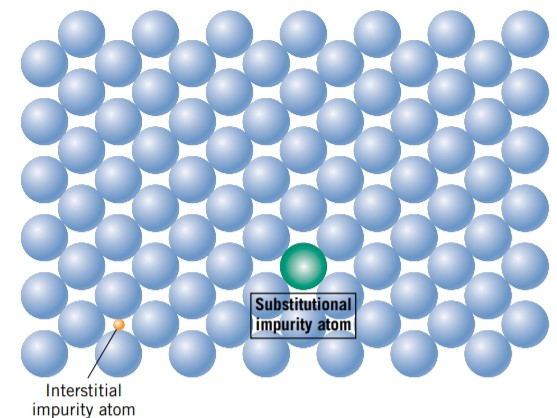
\includegraphics[width=7.7cm,height=5.5cm]{solucao-solida.jpg}
    \caption{Representação de impurezas substitucionais e intersticiais. Adaptado de \cite{callister2011materials}}
    \label{fig:solucao-solida}
\end{figure}

\pagebreak

Existem várias características que determinam o grau em que um elemento pode se solubilizar na rede \cite{callister2011materials}, são essas : 

\begin{itemize}
   \item Fator do tamanho atômico: Quando a diferença dos raios atômicos entre os dois tipos de átomos for menor que aproximadamente 15\%. Ao contrário os átomos com muita diferença no raio atômico que ocuparem as lacunas irão criar distorções substanciais na rede e uma nova fase irá se formar.
    \item Estrutura cristalina: Para que a solubilidade sólida seja considerável, as estruturas cristalinas dos metais de ambos os tipos de átomos devem ser as mesmas.
    \item Eletronegatividade: Quanto maior a eletronegatividade entre dois elementos, isto é, quanto mais eletropositivo for um elemento e mais eletronegativo for o outro, maior a probabilidade e formação de um composto intermetálico. Sendo assim, quanto menor a diferença de eletronegatividade entre dois componentes, maior a possibilidade de formar solução sólida.
    \item Valências: Sendo iguais todos os demais fatores, um metal apresentará maior tendência de dissolver um outro metal de maior valência.
\end{itemize}

Se esses três fatores abordados anteriormente não forem muito semelhantes, existe apenas uma solubilidade limitada. Este cenário pode ser descrito da seguinte maneira, em um solvente puro, alguns átomos são removidos e substituídos por átomos de soluto gradativamente, para aumentar a concentração de soluto. Eventualmente, no entanto, um nível de concentração máxima de soluto é atingido, e alguns átomos começam a ser rejeitados. Eles podem se agrupar para formar um pequeno cristal próprio, talvez com alguns átomos de solvente dissolvidos nele, ou reagir com alguns dos átomos de solvente para formar uma fase da estrutura do cristal diferente daquela de qualquer metal puro (ou seja, um metal intermetálico composto). No diagrama de fases as fases nas extremidades são denominadas terminal ou primária, e no centro do diagrama são denominadas as fases intermediárias. 

Soluções sólidas são definidas como substitucionais quando os elementos do soluto ocupam locais da rede que pertencem aos elementos do solvente, como no caso  do Níquel e Cobre que possuem apenas 2.5\% de diferença de raio atômico, apenas um elétron de diferença na camada de valência, e ambos apresentam estrutura cúbica de face centrada. Essa proximidade entre os dois elementos permite uma total solubilidade. Os átomos de níquel ocupam os locais da rede dos átomos de cobre e vice-versa indiscriminadamente para todas as composições, pode-se dizer que ambos formam uma série contínua de soluções sólidas. O diagrama de fases da liga binária Cu-Ni pode ser observado na Figura \ref{fig:diagrama-ni-cu}.

\pagebreak

\begin{figure}[ht]
    \centering
    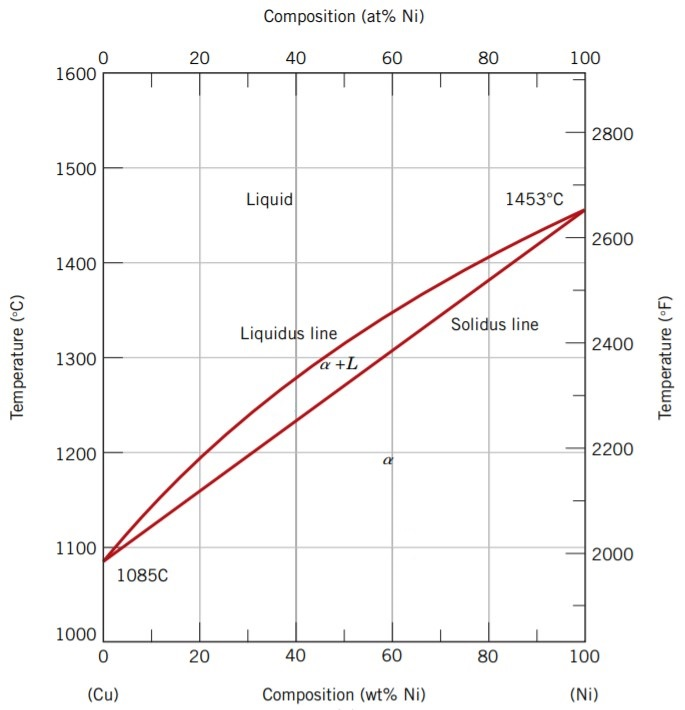
\includegraphics[height=8cm]{diagram-ni-cu.jpg} 
    \caption{Diagrama de fases Cobre-Níquel. Adaptado de \cite{callister2011materials} }
    \label{fig:diagrama-ni-cu}
\end{figure}


Algumas ligas metálicas em altas temperaturas apresentam solubilidade sólida completa, e quando submetidas a baixas temperaturas formam compostos intermetálicos. Porém, na grande maioria dos diagramas de fases de ligas metálicas conhecidas, o fenômeno de solubilidade sólida é relativamente restrito a pequenos intervalos de composição \cite{massalski1996structure}.

Soluções sólidas pode ser aleatórias, quando os elementos se distribuem na rede sem localização preferencial, ou podem ser ordenadas, quando determinados átomos diferentes apresentam certa afinidade. Se átomos da mesma natureza apresentarem afinidade, a formação de aglomerados tende a ocorrer, os quais podem distribuir de maneira ordenada ou aleatória\cite{massalski1996structure}. Exemplos de categorias de soluções sólidas estão demonstrados na Figura \ref{fig:modelo-ss} .

\begin{figure}[ht]
    \centering
    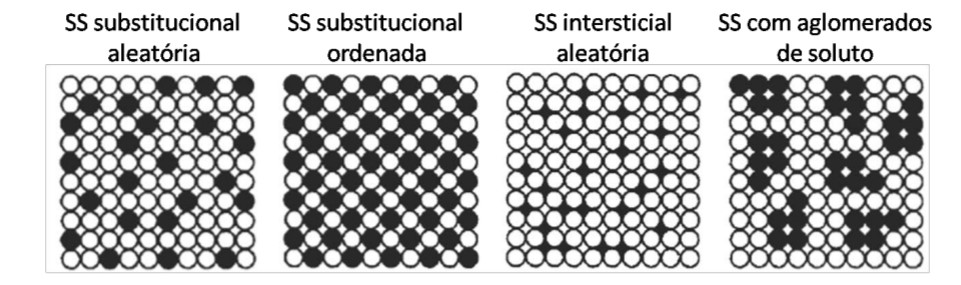
\includegraphics[width=12cm]{modelo-ss.jpg} 
    \caption{ Modelos esquemáticos de soluções sólidas. Adaptado de \cite{massalski1996structure}}
    \label{fig:modelo-ss}
\end{figure}

\pagebreak


\section{Termodinâmica}\label{sec:LABEL_CHP_2_SEC_A}

\subsection{Equilíbrio Termodinâmico}\label{sec:LABEL_CHP_2_SEC_A_SUB_A}


Uma parte de um sistema em que as propriedades e composição são homogêneas, e que é fisicamente distinta de outras partes do mesmo sistema pode ser definida como uma fase. Em um sistema composto por uma ou mais fases, o que diferencia cada parte deste sistema são seus componentes, isto é, diferentes elementos ou compostos químicos que constituem o sistema, assim como a composição de cada fase deste sistema pode ser definida como diferentes grupos de cada componente \cite{porter2009phase}.

Em um sistema com diferentes fases, elementos ou compostos químicos, é esperado que cada elemento tenha uma interação com os elementos que o rodeiam. Para um sistema ser considerado estável ou instável diversos fatores devem ser levados em conta, essa estabilidade relativa é estimada através da energia de livre de Gibbs, essa grandeza é determinada através da entalpia, entropia e da temperatura.

A energia livre de Gibbs de um sistema em que temos temperatura e pressão constantes, é dada pela Equação \ref{eq:gibbs}.

\begin{equation} 
G = H - TS
\label{eq:gibbs}
\end{equation}

Onde H é a entalpia, S é a entropia e T é a temperatura absoluta (K). Resumidamente temos que:

\begin{itemize}
  \item Quando $\Delta G < 0$ o processo é exergônico, ocorrerá de forma espontânea a formação de mais produtos.
  \item Quando $\Delta G > 0$ o processo é endergônico, ocorrerá de forma espontânea a formação de mais reagentes.
  \item Quando $\Delta G = 0$ o sistema está em equilíbrio e a concentração de produtos e reagentes permanecerão constantes. \cite{gaskell2012introduction}
\end{itemize}

\begin{table}[htb]
\centering
\caption{Espontaneidade quando $\Delta G < 0$ }
\begin{supertabular}{|m{2.0cm}|m{4.5cm}|m{4.5cm}|}
\hline
{  } &
{ $\Delta H < 0$ } &
{ $\Delta H > 0$ }\\\hline
{ $\Delta S > 0$ } &
{ Espontânea para todas T
( $\Delta G < 0$) } &
{ Espontânea para altas T
(quando $ T\Delta S$ é grande)
} \\\hline
{ $\Delta S < 0$ } &
{ Espontânea para baixas T
(quando $ T\Delta S$ é pequeno) } &
{ Não Espontânea para todas T
( $\Delta G > 0$) } \\\hline
\end{supertabular}
    \legend{}
    \label{quad:espontaneidade}
\end{table}

Considerando um sistema composto por átomos A e B em solução sólida. Cada átomo possui a sua respectiva energia livre de Gibbs, sendo assim ao considerar um sistema homogêneo em solução sólida dos elementos A e B, e que estes possuem a mesma estrutura cristalina, temos a energia livre de Gibbs deste sistema dada pela Equação \ref{eq:ss-mistura}:

\begin{equation} 
G = X_{A}G_{A} + X_{B}G_{B} + \Delta G_{mix}
\label{eq:ss-mistura}
\end{equation}

Onde $X_{A}$ e $X_{B}$ são as frações molares dos elementos A e B, $G_{A}$ e $G_{B}$ são as energias livres de Gibbs dos elementos A e B puros e $\Delta G_{mix}$ é a variação na energia livre de Gibbs devido à mistura dos átomos. Essa variável é determinada através da Equação \ref{eq:deltaG-mix}:

\begin{equation} 
\Delta G_{mix} = \Delta H_{mix} - T\Delta S_{mix}
\label{eq:deltaG-mix}
\end{equation}

Onde $\Delta H_{mix}$ é o calor envolvido durante a mistura dos elementos e $\Delta S_{mix}$ é a variação de entropia provocada pela mistura.

A entropia de uma solução sólida na termodinâmica estatística é quantificada através da aleatoriedade dada através da Equação \ref{eq:entropia-boltzmann}. Onde k é a constante de Boltzmann e $\omega$ é a medida de aleatoriedade. Essa entropia possui duas contribuições significativas, a contribuição térmica  e a contribuição configuracional. No caso da entropia térmica, a medida de aleatoriedade é dada pela quantidade de formas que a energia térmica de um sólido pode ser dividida entre os átomos, que é, a quantidade total de estados vibracionais de um sólido. Em soluções, devido as diferentes formas que os átomos podem ser arranjados existem também uma aleatoriedade adicional, isto nos leva a entropia configuracional, isto é, a o total de formas distintas em que os átomos de uma solução podem se organizar.

\begin{equation} 
 S =  k\ln \omega
\label{eq:entropia-boltzmann}
\end{equation}

Quando a variação de volume ou troca de calor durante a mistura é zero, a única contribuição para a entropia de mistura $\Delta S_{mix}$ será a entropia configuracional. 
\begin{equation} 
\omega_{config}=\frac{(N_{A} + N_{B})!}{N_{A}!N_{B}!}
\label{eq:entropia-config}
\end{equation}

Onde $N_{A}$ é a quantidade de átomos de A e $N_{B}$ a quantidade de átomos de B respectivamente. Uma vez que está sendo considerada uma solução de 1 mol, isto é, $N_{a}$ átomos (número de Avogadro), temos 
$N_{A}= X_{A}N_{a}$ e $N_{B}= X_{B}N_{a}$. Substituindo as equações (\ref{eq:entropia-boltzmann}) e (\ref{eq:entropia-config}) e usando a aproximação de Stirling ($\ln N! \simeq N \ln N - N$) e o relacionamento $N_{ak} = R$ (a constante universal dos gases) temos a entropia de mistura de uma solução sólida binária na Equação \ref{eq:entropia-mix} :

\begin{equation} 
\Delta S_{mix} = -R(X_{A}\ln X_{A} + X_{B}\ln X_{B})
\label{eq:entropia-mix}
\end{equation}


Uma vez que  $X_{A}$ e $X_{B}$ são valores menores que um, podemos concluir que há sempre um aumento na entropia do sistema devido à mistura dos elementos.

\subsection{Soluções Ideais}\label{sec:LABEL_CHP_2_SEC_A_SUB_B}

 A forma mais simples de mistura para de início é quando temos $\Delta H_{mix}=0$, consequentemente, segundo as Equações \ref{eq:deltaG-mix} e \ref{eq:entropia-mix}, temos a energia livre de Gibbs   \ref{eq:delta-gibbs}.

\begin{equation} 
\Delta G_{mix} = RT(X_{A}\ln X_{A} + X_{B}\ln X_{B})
\label{eq:delta-gibbs}
\end{equation}

Dessa forma, à partir das Equações \ref{eq:ss-mistura} e \ref{eq:delta-gibbs}, a energia livre de Gibbs do sistema pode ser definida pela Equação \ref{eq:livre-gibbs}:

\begin{equation} 
G=X_{A}G_{A} + X_{B}G_{B} + RT(X_{A}\ln X_{A} + X_{B}\ln X_{B})
\label{eq:livre-gibbs}
\end{equation}

Os valores de energia livre de Gibbs em função da variação de composição e
temperatura estão esquematizados na Figura \ref{fig:energia-livre-gibbs}, pode-se notar que para altas temperaturas, $G_{A}$ e $G_{B}$ ocorre uma redução significativa na energia livre de Gibbs de um sistema.

\begin{figure}[ht]
    \centering
    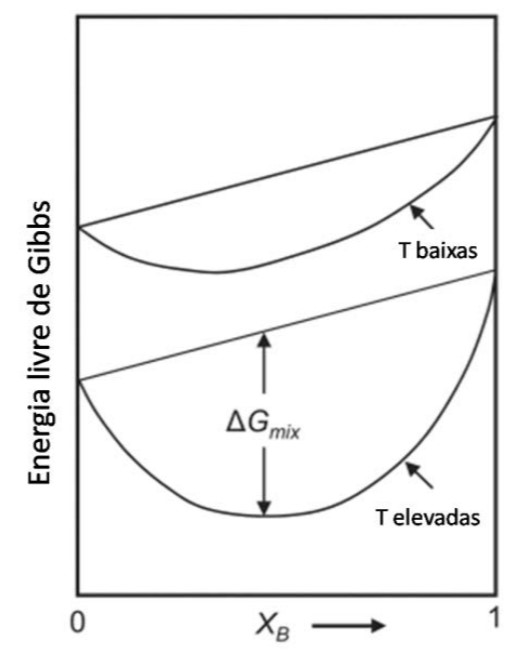
\includegraphics[height=7.5cm]{energia-livre-gibbs.jpg} 
    \caption{Energia livre de Gibbs de uma solução ideal. Adaptado de \cite{porter2009phase}.}
    \label{fig:energia-livre-gibbs}
\end{figure}

\subsection{Soluções Regulares}\label{sec:LABEL_CHP_2_SEC_A_SUB_C}

Analisando uma forma de mistura em que diferente do modelo ideal onde $\Delta H = 0$, temos um comportamento de contribuição da entalpia ($\Delta H \neq 0$) na energia livre de Gibbs, que na prática podemos observar uma mistura endotérmica (calor absorvido $\Delta H_{mix}>0$), ou uma mistura exotérmica (calor liberado $\Delta H_{mix}<0$). Novamente considerando os átomos A e B apresentando a as estruturas semelhantes, e que não a variação do volume durante a mistura, a entalpia de mistura será apenas função das energias de ligação entre os átomos adjacentes. Podemos considerar três possíveis energias de ligação neste modelo:
\begin{itemize}
  \item Ligações A--A, cada um com a energia $ \varepsilon_{AA}$, 
  \item Ligações B--B, cada um com a energia $ \varepsilon_{BB}$,
  \item Ligações A--B, cada um com a energia $ \varepsilon_{AB}$,
\end{itemize}

\begin{figure}[ht]
    \centering
    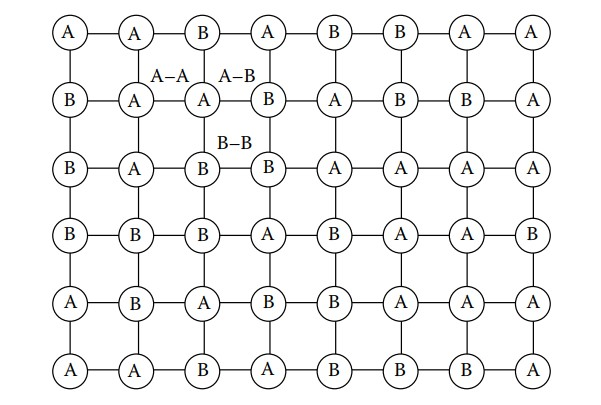
\includegraphics[height=7cm]{ligacoes.jpg} 
    \caption{Os diferentes tipos de ligações interatômicas em uma solução sólida. Adaptado de \cite{porter2009phase}.}
    \label{fig:ligacoes-interatomicas}
\end{figure}

A energia interna da solução E irá depender do número de ligações para cada tipo $P_{AA}$, $P_{BB}$ e $P_{AB}$: 
\begin{equation} 
E = P_{AA}\varepsilon_{AA} +  P_{BB}\varepsilon_{BB} + P_{AB}\varepsilon_{AB}
\label{eq:energia-interna-solucao}
\end{equation}
b
Antes de misturar, os elementos A e B puro, contém respectivamente as ligações A--A e B--B, e considerando a relação entre $P_{AA}$, $P_{BB}$ e $P_{AB}$, a mudança na energia interna da mistura é dada pela Equação \ref{eq:entalpia-ligacao}.
\begin{equation} 
\Delta H_{mix} = P_{AB} \varepsilon
\label{eq:entalpia-ligacao}
\end{equation}
Onde:
\begin{equation} 
\varepsilon = \varepsilon_{AB} - \frac{1}{2} ( \varepsilon_{AA} + \varepsilon_{BB})
\label{eq:energia-ligacao}
\end{equation}

Ou seja, $\varepsilon$ é a diferença entre a energia de ligação A--B e a média entre as energias de ligação de A--A e B--B. Sendo assim, se $\varepsilon=0$, $\Delta H_{mix}=0$ o que nos leva a solução ideal. No caso em que os átomos estão arranjados completamente aleatórios e a entropia de mistura é dada pela Equação \ref{eq:entropia-mix}. Então pode ser demostrado que:

\begin{equation} 
P_{AB} = N_{a}z X_{A}X_{B} \textrm{  ligações.mol}^{-1} 
\label{eq:energia-AB}
\end{equation}

Onde $N_a$ é o número de Avogadro e $z$ é o número de ligações por átomo. Se $\varepsilon<0$ os átomos na solução irão dar preferência a fazer ligações com o átomo oposto, resultando no aumento de $P_{AB}$, enquanto que, se $\varepsilon>0$, $P_{AB}$ será menor do que numa solução aleatória. Considerando que $\varepsilon$ não é tão diferente de zero, podemos reescrever a Equação \ref{eq:energia-AB}:

\begin{equation} 
\Delta H_{mix} = \Omega X_{A}X_{B}
\label{eq:entalpia-mistura}
\end{equation}

Onde:

\begin{equation} 
\Omega = N_{a}z \varepsilon
\label{eq:omega}
\end{equation}

Sendo assim podemos determinar os valores da energia livre de Gibbs em função de $\Omega$ e da temperatura, substituindo a Equação \ref{eq:deltaG-mix} por  \ref{eq:entropia-mix} e  \ref{eq:entalpia-mistura} temos que:

\begin{equation} 
\Delta G_{mix} = \Omega X_{A}X_{B} + RT(X_{A}\ln X_{A} + X_{B}\ln X_{B})
\label{eq:deltaG-mix-regular}
\end{equation}


A equação \ref{eq:deltaG-mix-regular} pode ser representada na figura \ref{fig:gibbs-temperatura-composicao}, em diferentes valores de $\Omega$ e de temperatura, temos diferentes comportamentos na entropia e entalpia e consequentemente alterando a energia livre de Gibbs. 

\begin{figure}[ht]
    \centering
    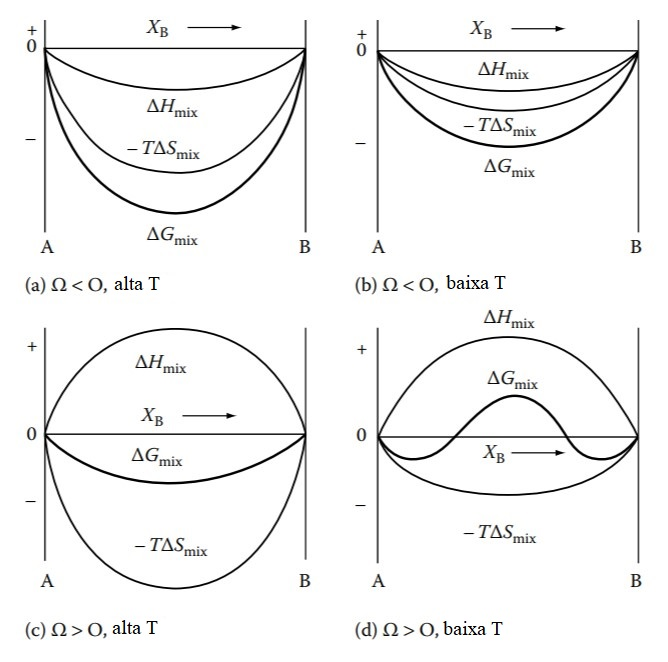
\includegraphics[height=12cm]{gibbs-temperatura-composicao2.jpg} 
    \caption{Resultado da influência da temperatura, composição e número de ligações nos valores da energia de Gibbs, entalpia e entropia. Adaptado de \cite{porter2009phase}.}
    \label{fig:gibbs-temperatura-composicao}
\end{figure}

\pagebreak

De acordo com a Figura \ref{fig:gibbs-temperatura-composicao} é observado que quando a composição $X_{A}$ e $X_{B}$ são iguais, isto é, quando a composição se torna equiatômica, a energia livre de Gibbs atinge seu menor valor. Consequentemente em ligas com composição equiatômica quando em solução sólida, tendem a apresentar fases estáveis, possibilitando uma composição de fase homogênea do material produzido.

Em um cenário ideal a confecção de ligas com a composição equiatômica, possibilitaria desenvolver um material com propriedades significativamente superiores aos materiais de ligas convencionais de uma matriz com elemento dominante. Porém a explicação abordada anteriormente se refere a um caso simples com apenas dois elementos. Ao se tratar de uma liga mais complexa com cinco ou mais elementos, os parâmetros para definição da energia livre de Gibbs se tornam mais complexos, e quando a entalpia de mistura é diferente de zero, nem sempre o equiatomicidade resultará na menor energia livre de Gibbs, isto devido a interferência da energia de ligação interatômica. Neste caso quando é observado um comportamento em que a energia de ligação supera a energia livre de Gibbs  há a formação de compostos intermetálicos \cite{porter2009phase}.

\pagebreak

\section{Ligas de alta entropia}\label{sec:LABEL_CHP_3_SEC_A}


Conhecidas também pelo termo inglês (HEAs - High-entropy alloys), são materiais altamente avançados que diferentemente das ligas convencionais, as HEAs possuem múltiplos elementos principais na liga, frequentemente cinco ou mais elementos de peso e raio atômico quase iguais. O princípio básico por trás de uma HEA é a capacidade das fases de solução sólida serem relativamente estáveis, devido a sua alta entropia de mistura, a estabilização da solução sólida é significativamente maior do que a formação de intermetálicos. Basicamente as HEAs contém ao menos cinco elementos e a composição atômica de cada elemento varia entre 5\% e 35\%. \cite{yeh2013alloy} \cite{yeh2004nanostructured}

\begin{figure}[ht]
    \centering
    
\includegraphics{esquema-ligas-hea.png} 
    \caption{Esquema de uma liga de alta entropia composta por cinco elementos em matriz de solução sólida}
    \label{fig:esquema-ligas-hea}
\end{figure}


Baseando-se na equação de Boltzmann \cite{gaskell2012introduction}, relacionando a entropia e a complexidade do sistema \cite{thermodynamicsOfSolid}, a mudança de entropia configuracional por mol, $\Delta S_{config}$, durante a formação de uma solução  de n elementos com frações equimolares pode ser calculada a partir da seguinte equação:

\begin{equation}
    \Delta S_{config} = k \ln \omega
\end{equation}

onde k é a constante de Boltzmann e $\omega$ é a medida de aleatoriedade para energia disponível na mistura ou dispersa entre as partículas de um sistema. Assim a entropia configuracional em função do número de moles de uma solução sólida de n elementos com fração molar de $x_i$ é:

\begin{equation}
    \Delta S_{config} = - R \sum_{i=1}^{n} X_{i} \ln X_{i}
\end{equation}

Considerando uma liga equiatômica no estado líquido ou em uma solução sólida regular. A entropia configuracional por mol é dada pela Equação \ref{eq:boltzmman-complexidade} \cite{yeh2004nanostructured} \cite{yeh2013alloy}:
\begin{equation} 
\Delta S_{config} = - k \ln \omega = - R (\frac{1}{n} \ln \frac{1}{n} + \frac{1}{n} \ln \frac{1}{n} + ... + \frac{1}{n} \ln \frac{1}{n}) = -R \ln \frac{1}{n} = R \ln n
\label{eq:boltzmman-complexidade}
\end{equation}

Onde R é a contante dos gases igual a $8,314J/K^{-1}mol^{-1}$.  Pela regra de Richard \cite{thermodynamicsOfSolid}, as mudanças de entropia na fusão da maioria dos metais são apenas empiricamente igual a R em seus pontos de fusão.
A entropia configuracional de ligas equiatômicas em função dos elementos principais é demonstrado na tabela \ref{quad:entropia-config-n} e na figura \ref{fig:entropia-configuracional-elementos}.


\begin{table}[htb]
\centering
\caption{Entropia configuracional de ligas equimolares para n elementos}
\begin{supertabular}{|m{1.5cm}|m{1.5cm}|m{1.5cm}|m{1.5cm}|m{1.5cm}|m{1.5cm}|m{1.5cm}|m{1.5cm}|}
\hline
{ n } &
{ 1 } &
{ 3 } &
{ 5 } &
{ 7 } &
{ 9 } &
{ 11 } &
{ 13 }\\\hline
{ $\Delta S_{config}$ } & 
{ 0 } &
{ 1,10R } &
{ 1,61R } &
{ 1,95R } &
{ 2,20R } &
{ 2,40R } &
{ 2,57R} \\\hline
\end{supertabular}
    \legend{}
    \label{quad:entropia-config-n}
\end{table}

\begin{figure}[ht]
    \centering
    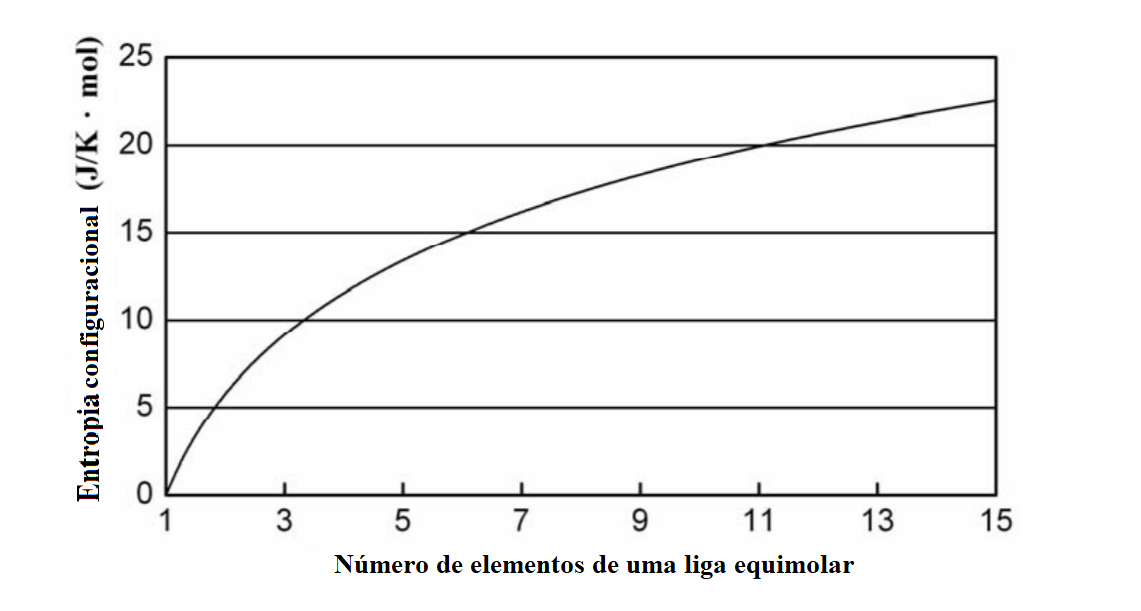
\includegraphics[height=6cm]{entropia-mistura-numero-elementos.png} 
    \caption{Entropia configuracional em função do número de elementos para ligas equimolares. Adaptado de \cite{jien2006recent}.}
    \label{fig:entropia-configuracional-elementos}
\end{figure}

Por convenção, uma liga é considerada de alta entropia quando possui a entropia configuracional maior que 1,5R. sendo assim uma liga de alta entropia é classificada conforme a figura \ref{fig:divisao-ligas-alta-entropia} \cite{gao2016high}:

\begin{figure}[ht]
    \centering
    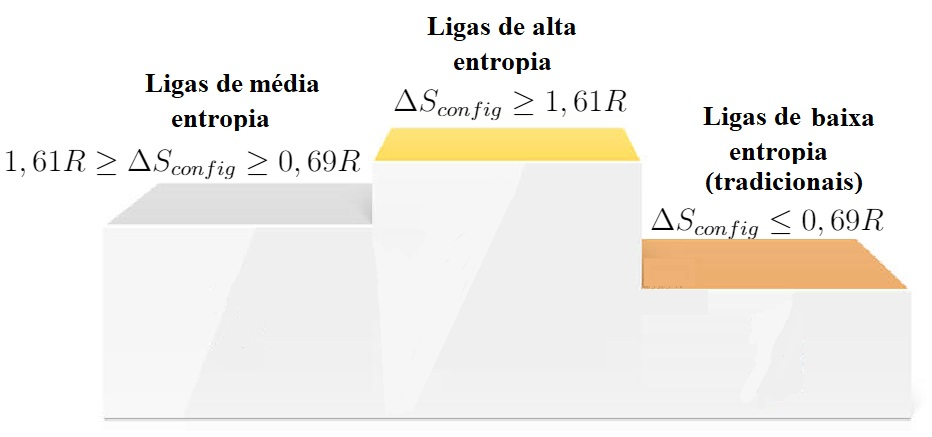
\includegraphics[height=6cm]{divisao-ligas-alta-entropia.jpg} 
    \caption{Divisão das ligas baseado na entropia configuracional.}
    \label{fig:divisao-ligas-alta-entropia}
\end{figure}
     
\pagebreak
                   
\subsection{Efeitos principais em Ligas de Alta Entropia}\label{sec:LABEL_CHP_3_SEC_B_SUB_A}

Em ligas de alta entropia, existem muitos fatores que afetam a microestrutura e as suas propriedades. Dentre estes diversos fatores, quatro deles se destacam \cite{yeh2013alloy}, são eles a alta entropia, distorção severa da rede, difusão retardada e efeito coquetel \cite{gao2016high} \cite{murty2019high}.

\subsection{Alta Entropia}\label{sec:LABEL_CHP_3_SEC_B_SUB_B}

É o efeito mais importante em Ligas de Alta Entropia, este contribui com o aumento da formação de fases em solução sólida, tornando a microestrutura muito mais simples do que a conhecida em ligas convencionais. Há três categorias de estados concorrentes no estado sólido de uma liga, isto é, fases elementares, compostos intermetálicos e fases de solução sólida. 
A competição envolvendo a fase líquida durante a solidificação não é considerada. A fase elemental é a fase terminal de uma solução sólida baseada em um único elemento metálico. 
Compostos intermetálicos são compostos estequiométricos que possuem super redes específicas, como NiAl e Ni$_{3}$ Ti. Solução sólida é a fase de mistura completa de todos os elementos ou com uma mistura significante em que elementos constituintes da liga apresentam a mesma estrutura cristalina. Fases intermetálicas ou intermediárias estão inclusas também porque são solidas baseadas em componentes intermetálicos. Nessas fases, diferentes elementos constituintes tendem a ocupar diferentes conjuntos de locais de rede. De acordo com a Segunda lei da Termodinâmica, o estado com a menor energia livre de mistura $\Delta G_{mix}$ entre todos os possíveis estados deve estar em estado de equilíbrio. 
Em resumo, o efeito de alta entropia é importante para Ligas de Alta Entropia para evitar a formação de muitos tipos diferentes de compostos estequiométricos, que são muito frágeis e complexos. Por outro lado, promove a formação de solução sólida, reduzindo o número de fases conforme previsto pela regra de fase de Gibbs, que permite que o número de fases em equilíbrio aumente com o número de componentes. \cite{yeh2013alloy}


% A figura 1 abaixo representa o diagrama ternário da entropia de mistura de um sistema de uma liga ternária $\Delta S_{mix}(J.mol^{-1}K^{-1})$. As regiões de cor azul indicam a presença de ligas convencionais baseadas em um ou dois elementos principais, e a região vermelha do centro indica  alta entropia.

% \begin{figure}[ht]
%     \centering
%     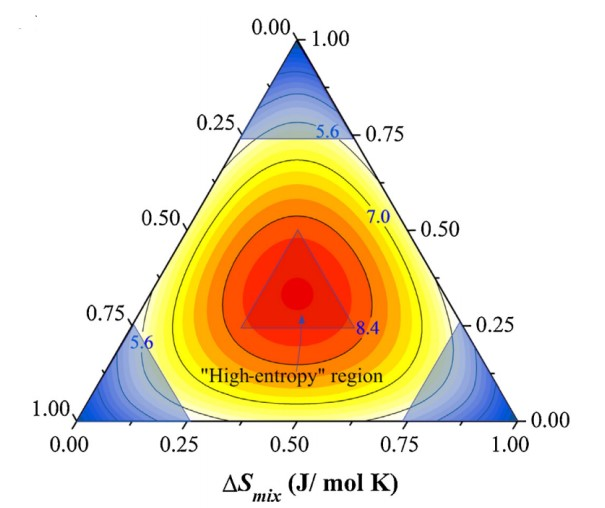
\includegraphics[width=8.5cm,height=7.5cm]{diagrama-ternario-de-entropia.jpg}
%     \caption{Esquema de um sistema de liga ternária . Adaptado de  \cite{ye2016high}}
%     \label{fig:internet}
% \end{figure}




\subsection{Distorção severa na rede}\label{sec:LABEL_CHP_3_SEC_B_SUB_C}

Devido a uma matriz multielementar, cada fase em solução sólida em uma Liga de Alta Entropia é uma  inteiramente composta por solutos \cite{tong2005mechanical}, onde cada átomo está rodeado por diferentes tipos de elementos, e consequentemente, apresentando tensões e deformações na rede devido a diferença de raio atômico entre  eles.

Além da diferença de raio atômico, tanto a diferença de energia de ligação quanto a tendencia de estrutura cristalina entre os elementos constituintes também podem causar distorções ainda maiores na rede, isto porque as ligações não simétricas e a estrutura eletrônica estão presentes entre um átomo e seus primeiros vizinhos, além dessa assimetria variar de local para local na rede.\cite{tsai2013sluggish}\cite{yeh2007anomalous} 

\begin{figure}[ht]
    \centering
    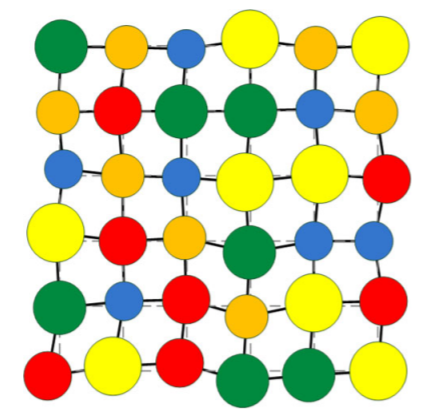
\includegraphics[width=8.5cm,height=7.5cm]{distorcao-severa-rede.png} 
    \caption{Distorção severa na rede cristalina devido a diferença de tamanho e energia de ligação dos elementos. Adaptado de \cite{yeh2013alloy}}
    \label{fig:internet}
\end{figure}

A gravidade do efeito da distorção na rede é significativamente maior em ligas de alta entropia, quando comparadas as ligas convencionais, isto porque em ligas convencionais a maioria dos átomos da matriz possuem o mesmo tipo de átomos em sua vizinhança.

Segundo \cite{yeh2013alloy} essa distorção não afeta apenas as propriedades, como também reduz o efeito térmico sobre a liga. A dureza e a resistência mecânica aumentam efetivamente devido ao grande endurecimento da solução na rede fortemente distorcida. Foi observado que ligas com a estrutura CFC são menos endurecíveis por solução sólida quando comparadas a ligas com estrutura CCC \cite{brooks1982heat}. Na estrutura CFC, cada átomo é cercado por 12 átomos vizinhos, por outro lado, na estrutura CCC, cada átomo é cercado por 8 átomos. Dessa maneira, considerando a o mesmo conjunto de elementos, um átomo na estrutura CFC terá maior probabilidade de estar ligado com o mesmo elemento, resultando, assim, em menor endurecimento e menor distorção na rede\cite{dieter1976mechanical}.

Outro fenômeno que vale ressaltar é a queda significativa da condutividade elétrica observada em ligas de Alta Entropia, isto ocorre por causa do espalhamento de elétrons ocasionado pela distorção da rede. Que por consequência influi na redução da condutividade térmica \cite{kao2011electrical}.

% \begin{figure}[ht]
%     \centering
%     \caption{Distorção severa em rede de uma estrutura cristalina multielementar}
%     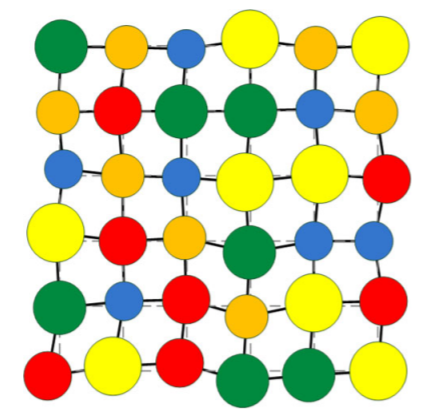
\includegraphics{distorcao-severa-rede.png} 
%     \legend{Fonte: Yeh, Alloy design strategies and future trends in high-entropy alloys (2013, p. 1764)}
%     \label{fig:internet}
% \end{figure}


\pagebreak

\subsection{Difusão lenta}\label{sec:LABEL_CHP_3_SEC_B_SUB_D}

Em ligas de alta entropia, a concentração de lacunas na rede é limitada quando comparado a ligas tradicionais, isso porque cada lacuna está associada a entalpia positiva de formação e excesso de entropia de mistura, na qual gera uma mínimo de energia livre de mistura a uma certa concentração de equilíbrio para uma dada temperatura. \cite{thermodynamicsOfSolid}


Uma lacuna em uma solução sólida é rodeada e competida por átomos de diferentes elementos durante a difusão. Foi proposto que a difusão mais lenta e alta energia de ativação ocorre em Ligas de Alta Entropia devido à grande flutuação da energia potencial da rede entre os locais da rede. É considerado que a difusão lenta e a alta energia de ativação pode ocorrer em HEAs devido a abrangente variação da energia potencial da rede entre sítios da rede.\cite{tsai2013sluggish}. Tudo isso, somado à distorção severa da rede, a qual limita a movimentação atômica, resultando numa taxa de difusão limitada em ligas de alta entropia \cite{jien2006recent}.

Devido ao efeito de difusão lenta, vantagens são fornecidas pelo fato de afetar diretamente na nucleação, crescimento de grão de forma mais lenta, precipitados nanométricos, temperatura de recristalização elevada e aumento da resistência a fluência. Essas vantagens trazem benefícios para o controle da microestrutura \cite{gao2016high}.


\subsection{Efeito coquetel}\label{sec:LABEL_CHP_3_SEC_B_SUB_E}

O termo ``coquetel multimetálico'' foi utilizado na literatura para enfatizar o aprimoramento das propriedades das ligas metálicas através da utilização de cinco ou mais elementos principais. Esse efeito indica que propriedades inesperadas podem ser
obtidas através da combinação de múltiplos elementos em uma liga, propriedades essas
que não poderiam ser obtidas em ligas baseadas em um único elemento principal

Apesar de sua grande tendência em possuir microestrutura monofásica, ligas de alta
entropia podem apresentar mais de uma fase, dependendo de sua composição e rota de 
processamento. Como em qualquer liga metálica, suas principais propriedades são
ditadas pelas fases que a constituem, através do efeito da morfologia, distribuição,
contornos e propriedades dessas fases. Cada fase consiste em uma solução sólida
multielementar, que pode ser definida como um compósito se analisada em escala
nanométrica. As propriedades desse compósito são regidas não somente pelas
propriedades básicas de cada elemento, mas também pela interação entre os mesmos e
pela distorção severa da rede. De maneira geral, o efeito coquetel vai desde a escala
atômica, através do efeito de compósito multielementar, até a escala micrométrica, pelo
efeito de multifases.


\pagebreak

\section{Aprendizado de Máquina e Algoritmos}\label{sec:LABEL_CHP_4_SEC_A}


Conhecido também pelo termo em inglês Machine Learning, é a capacidade da máquina através de um algoritmo computacional, desempenhar funções cognitivas geralmente associadas a mente humana, tais como aprender, identificar padrões e resolver problemas complexos\cite{michalski2013machine}. O aprendizado de máquina tem como principal objetivo extrair informações de dados fornecidos, e então desenvolver um modelo genérico suficiente, que é capaz de responder de maneira apropriada um problema proposto.

O aprendizado de máquina pode ser agrupado em três categorias: Aprendizado Supervisionado, Não Supervisionado e Reforçado. Além disso, esses grupos podem ser subclassificados como Aprendizado Passivo ou Aprendizado Ativo. Um algoritmo pode ser do tipo Supervisionado Passivo ou Supervisionado e Ativo, por exemplo.

Algumas das principais etapas do aprendizado de máquina estão no fluxograma da Figura \ref{fig:tipos-aprendizado},  além disso essas atividades são usadas em diferentes tipos de aprendizado, que serão discutidos a seguir.


\begin{figure}[ht]
    \centering
    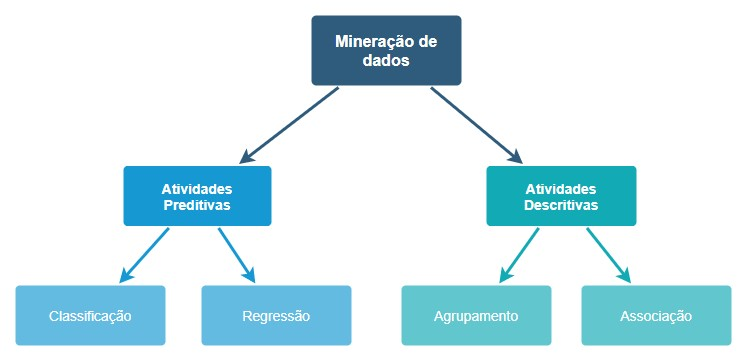
\includegraphics[height=7.5cm]{tipos-aprendizado.jpg} 
    \caption{Atividades de aprendizado de máquina}
    \label{fig:tipos-aprendizado}
\end{figure}

\pagebreak

\subsection{Aprendizado supervisionado}\label{sec:LABEL_CHP_4_SEC_A_SUB_A}

No aprendizado supervisionado supõe-se que os objetos de uma categoria ou classe compartilham características comuns, semelhantes, que proporcionam informações suficientes para o algoritmo conseguir distinguir e classificar uma nova informação não observada antes. Um especialista é responsável por preparar os parâmetros de entrada do algoritmo e observar o resultado de saída, e avaliar se a resposta obtida pelo modelo condiz com o esperado, e caso necessário o especialista ajusta novamente os parâmetros do modelo, a Figura \ref{fig:aprendisado-supervisionado} ilustra esse conceito.



\begin{figure}[ht]
    \centering
    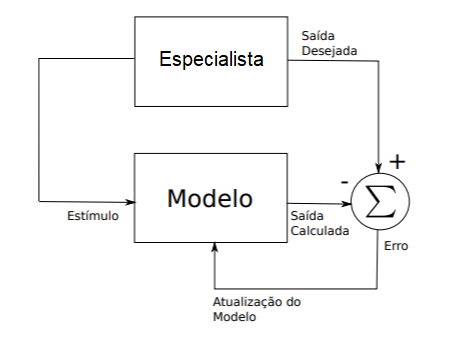
\includegraphics[height=5.2cm]{aprendizado-supervisionado.png} 
    \caption{ Aprendizado Supervisionado. Adaptado de \cite{de2007redes}}
    \label{fig:aprendisado-supervisionado}
\end{figure}

Neste aprendizado temos basicamente a regressão e a classificação \cite{dangeti2017statistics}. Na regressão o valor a ser previsto é uma variável numérica contínua, como por exemplo, o preço de um imóvel, temperatura prevista para uma data. E na classificação, será previsto uma categoria, como por exemplo se um e-mail é spam ou não, se um caractere em uma imagem é uma letra ou numero, ou para o caso deste trabalho qual a fase esperada para uma determinada composição de uma liga.

\subsection{Aprendizado não supervisionado}\label{sec:LABEL_CHP_4_SEC_A_SUB_B}

No aprendizado não supervisionado os dados são utilizados para estímulo do algoritmo, isto é, para treinamento do modelo, podem ou não estar acompanhados dos dados desejados para a saída. Além disso, nesse caso não há a figura do ``especialista'' e não é feito nenhum procedimento de correção do erro (Figura \ref{fig:aprendizado-nao-supervisionado}). O modelo observa os padrões e correlações das informações disponibilizadas e agrupa o conjunto de dados em classes.

\begin{figure}[ht]
    \centering
    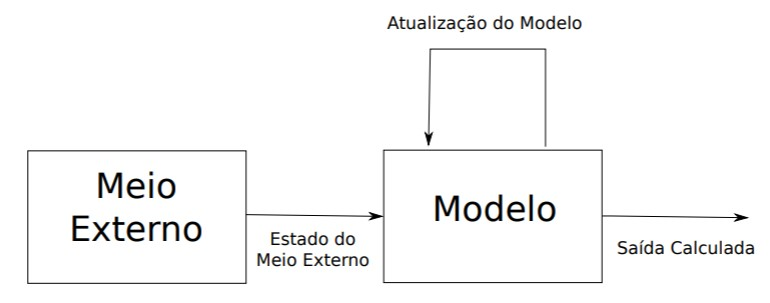
\includegraphics[height=4.2cm]{aprendizado-nao-supervisionado.jpg} 
    \caption{ Aprendizado não supervisionado. Adaptado de \cite{de2007redes}}
    \label{fig:aprendizado-nao-supervisionado}
\end{figure}
\FloatBarrier

\subsection{Aprendizado por reforço}\label{sec:LABEL_CHP_4_SEC_A_SUB_C}

O aprendizado por reforço é um mecanismo onde o modelo segue um ciclo baseado em observação, ação, recompensa e novo estado, pode ser descrito como um processo de Markov \cite{fernando2020cadeiaMarkov}, este processo possui as seguintes informações:

\begin{itemize}
    \item E:  espaço de estados
    \item A:  espaço de ações
    \item R:  função de recompensas \\
    $R(e,a): E \times A \rightarrow \mathbb{R}$
    \item T:  função de transição de estado \\ 
    $T(e,a,e'): E^2 \times A \rightarrow [0,1]$ \\
    $T(e,a,e') = p(e'|e,a)$
    \item $\gamma$: fator de ajuste entre recompensas de curto e longo prazo
\end{itemize}


O principal objetivo é maximizar a recompensa obtida a partir de uma função de escolha $\pi(e): E \rightarrow A$

\begin{figure}[ht]
    \centering
    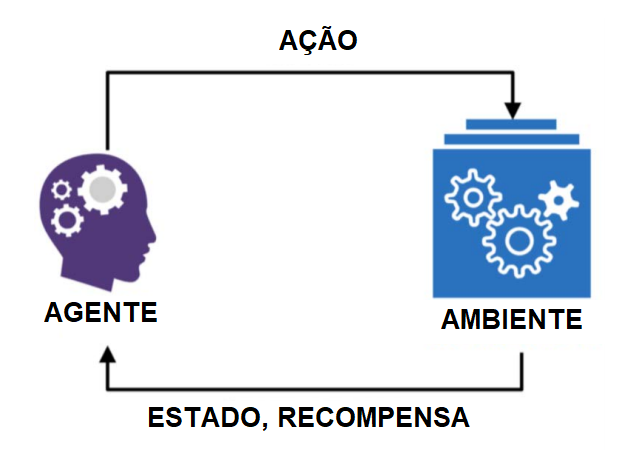
\includegraphics[height=6cm]{aprendizado-reforcado.png} 
    \caption{ Aprendizado reforçado.}
    \label{fig:aprendizado-reforcado}
\end{figure}
\FloatBarrier


\subsection{Classificação}\label{sec:LABEL_CHP_4_SEC_A_SUB_D}


Um problema é linearmente separável se existe um hiperplano capaz de separar completamente as classes. Quanto maior a separabilidade das classes, menor a complexidade do problema \cite{smola2008introduction}, na Figura \ref{fig:complexidade-sistema} pode-se observar os tipos de complexidade de dados.

\begin{figure}[ht]
    \centering
    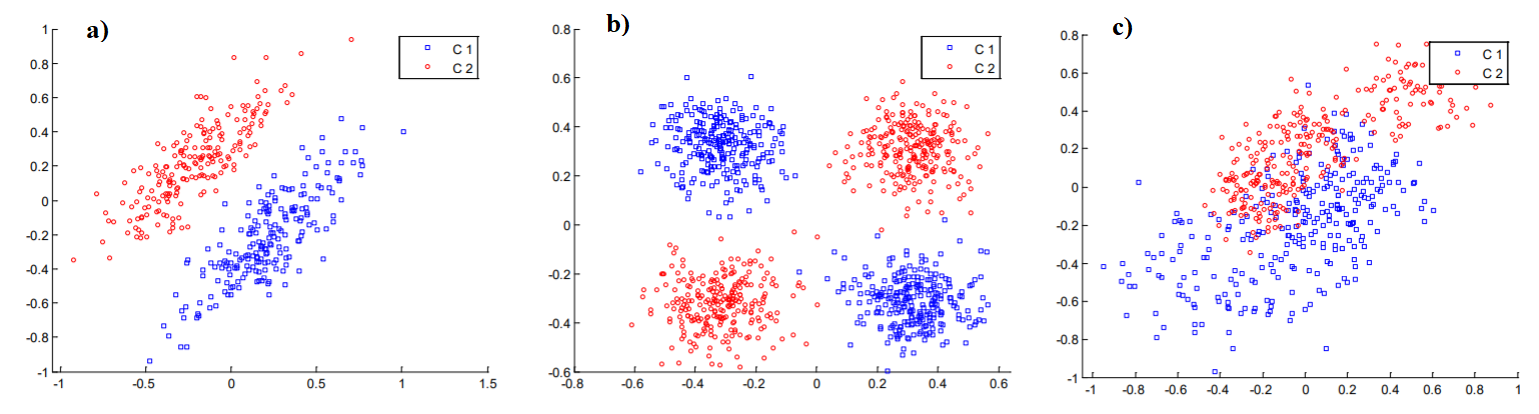
\includegraphics[height=4.2cm]{complexidade-sistema.png} 
    \caption{ a) Linearmente separável b) Separável não linearmente c) Não separável}
    \label{fig:complexidade-sistema}
\end{figure}
\FloatBarrier

Um algoritmo classificador possui a capacidade de rotular uma nova informação proposta ao modelo baseando-se no padrão dos dados de um conjunto previamente observado. Além disso para mensurar a qualidade do algoritmo classificador são realizadas algumas avaliações como a performance, precisão, acurácia e outras métricas de avaliação do mesmo.




\subsection{Regressão}\label{sec:LABEL_CHP_4_SEC_A_SUB_E}

 O objetivo da regressão é o desenvolvimento de um modelo capaz de identificar o valor mais correto possível para um novo conjunto de entradas.



\begin{figure}[ht]
    \centering
    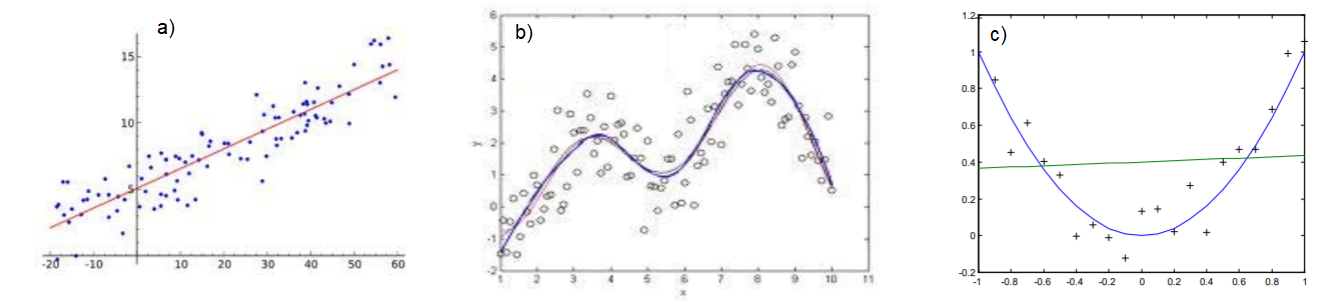
\includegraphics[width=16cm]{regressoes.png} 
    \caption{ a) Linear b) Não Linear c) Polinomial}
    \label{fig:regressoes}
\end{figure}
\FloatBarrier

\pagebreak
\subsection{Ajuste de modelo}\label{sec:LABEL_CHP_4_SEC_A_SUB_F}

Quando algoritmos de aprendizado de máquina são construídos, o conjunto de dados de uma amostra é utilizado para treinar o modelo. No entanto, dependendo de da forma que o modelo foi ajustado aos dados, como por exemplo, o tempo de treinamento, a complexidade do modelo, falta ou excesso de variáveis, poderá ocorrer consequências nos resultados se não houver um equilíbrio no ajuste do modelo, isto é, um cenário de underfitting ou overfitting.

\begin{figure}[ht]
    \centering
    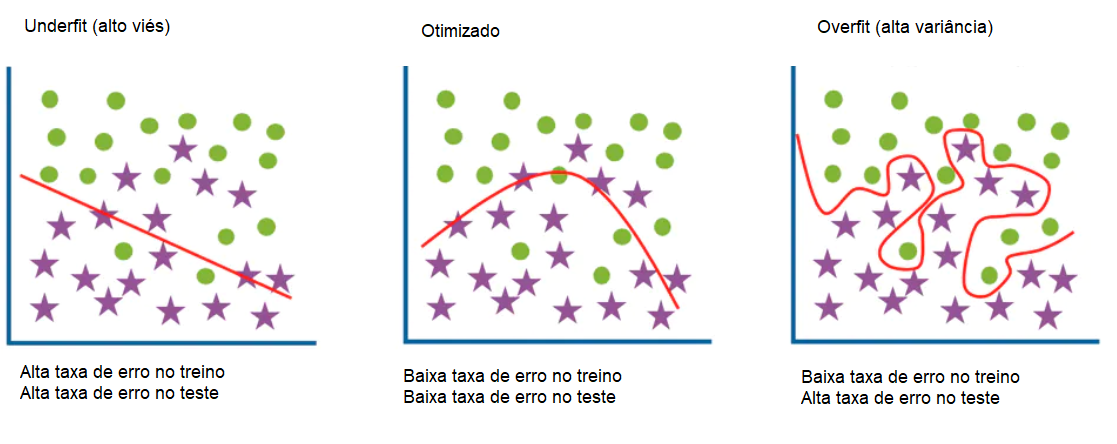
\includegraphics[height=6cm]{overfitting-underfitting.png} 
    \caption{Overfitting vs. underfitting. Adaptado de \cite{art:overfitting} }
    \label{fig:fitting-underfitting}
\end{figure}
\FloatBarrier

Em ambos os cenários, o modelo não é capaz de estabelecer a tendência dominante no conjunto de dados de treinamento. Como resultado, o underfitting também generaliza mal para dados não vistos. No entanto, ao contrário do overfitting, os modelos subajustados apresentam alta polarização e menos variação em suas previsões. Isso demonstra a relação inversamente proporcional de viés-variância, que ocorre quando um modelo subajustado muda para um estado superajustado. À medida que o modelo aprende, seu viés reduz, mas pode aumentar a variância à medida que se torna excessivamente ajustado. Ao ajustar o modelo, o objetivo é encontrar o ``ponto ideal'' entre sub e sobre ajuste, para que possa estabelecer uma tendência dominante e aplicá-la amplamente a novos conjuntos de dados.

\subsubsection{Overfitting}\label{sec:LABEL_CHP_4_SEC_A_SUB_F_A}
Overfitting é um conceito em ciência de dados, onde, um modelo é ajustado excessivamente e começa a aprender o ``ruído'', ou informação irrelevante, dentro do conjunto de dados. Quando isso acontece, o algoritmo se torna incapaz de classificar ou prever dados nunca antes vistos, isso significa uma baixa generalização do modelo. 

Baixas taxas de erro e alta variância são bons indicadores de overfitting. Para evitar esse tipo de comportamento, parte do conjunto de dados de treinamento é separada como um ``conjunto de teste'' para verificar a ocorrência de overfitting. Quando os dados de treinamento apresentarem baixa taxa de erro, e os conjunto de teste tiverem uma alta taxa de erro, é um claro sinal de overfitting.

\subsubsection{Underfitting}\label{sec:LABEL_CHP_4_SEC_A_SUB_F_B}
Por outro lado, quando é observado underfitting, o modelo não é capaz de capturar a relação entre as variáveis de entrada e saída com precisão, resultando numa alta taxa de erros em tanto para o conjunto de treinamento quanto para dados não vistos. Isso ocorre quando um modelo é muito simples, é resultado de um modelo que precisa de mais tempo de treinamento, mais recursos de entrada, ou menos regularização. Assim como o overfitting, é o mal ajuste de um modelo, onde ele não é capaz de estabelecer uma tendência na maioria dos dados, e consequentemente, resultando em erros no treinamento e baixo desempenho no modelo ao classificar ou prever dados novos.


\subsection{Validação cruzada}\label{sec:LABEL_CHP_4_SEC_A_SUB_G}

Avaliar um conjunto de dados de tamanho limitado é uma tarefa muito desafiadora. Ao separar o conjunto de dados em treino e teste, podemos ter overfitting no conjunto de testes porque os parâmetros podem ser ajustados até que o estimador tenha um desempenho ideal. Isto significa que o conjunto de teste deixa de representar uma amostra generalizada. Para contornar essa situação, podemos separar uma outra parte do conjunto de dados para ser o ``conjunto de validação'': o treinamento continua no conjunto de treinamento, logo após é utilizado o conjunto de validação para verificar se o ajuste do modelo foi bem sucedido, e por fim é feita a avaliação do modelo com o conjunto de teste.

No entanto, ao particionar o conjunto de dados em três conjuntos, reduzimos drasticamente o número de amostras disponíveis para o treinamento do modelo, isto é uma penalidade ainda maior quando consideramos um conjunto de dados bastante limitado.

\pagebreak

Uma solução para esse problema é o uso da validação cruzada (também conhecida como cross validation em inglês). Neste caso um conjunto de teste ainda é utilizado na avaliação final, porém não é necessário o uso de um conjunto de validação. O conjunto de treinamento é dividido em $k$ conjunto menores, então o modelo é treinado com $k-1$ das divisões do conjunto, porém em $k$ etapa do treinamento o conjunto de teste é diferente\cite{art:cross-validation}.


\begin{figure}[ht]
    \centering
    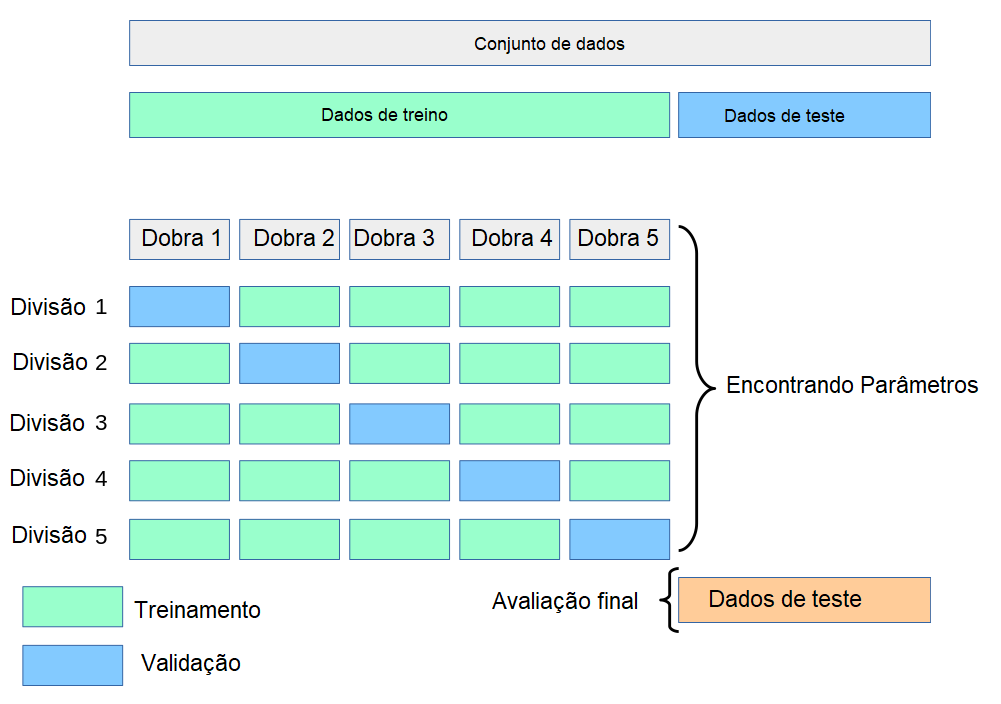
\includegraphics[height=8cm]{grid_search_cross_validation.png} 
    \caption{Ciclos do algoritmo de validação cruzada}
    \label{fig:crossv}
\end{figure}
\FloatBarrier



\subsection{Métricas de avaliação}\label{sec:LABEL_CHP_4_SEC_A_SUB_H}

Após criarmos um modelo de classificação, é necessário verificar a qualidade do modelo, para isso, são utilizadas algumas métricas, que por sua vez, usam a relação entre a previsão do modelo e os dados reais dando origem a uma matriz de confusão (Figura \ref{fig:matriz_confusao}).

\begin{figure}[ht]
    \centering
    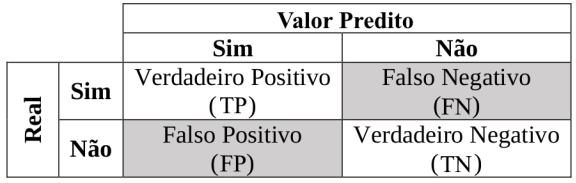
\includegraphics[height=4cm]{matriz_confusao.png} 
    \caption{Matriz de confusão}
    \label{fig:matriz_confusao}
\end{figure}
\FloatBarrier

\begin{itemize}
    \item Positivo Verdadeiro (True Positive – TP) que significa que a classe prevista e observada originalmente fazem parte da classe positiva;
    \item Falso Positivo (False Positive – FP) que significa que a classe predita retornou positivo mas a original observada era negativa;
    \item Negativo Verdadeiro (True Negative – TN) os valores preditos e observados fazem parte da categoria negativa;
    \item Falso Negativo (False Negative – FN) representa que o valor predito resultou na classe negativa mas o original observado era da classe positivo.
\end{itemize}

Com base nos resultados da matriz de confusão os valores das métricas podem ser calculados.

\begin{itemize}
    \item Acurácia (Acurary): Quantidade classificada como Positivos e Negativos corretamente, e pode ser formalizada em (TP + TN) / (TP + TN + FP + TN)
    \item Precisão (Precision): Quantidade Positiva classificada corretamente. E é calculada por TP / (TP + FP)
    \item Recall: Taxa de valores classificada como Positivo, comparada com quantos deveriam ser. E pode ser calculada como  \\
    $TP / (TP + FN)$
    \item F1 SCORE: É calculado como a média harmônica entre Precisão e Recall, sendo sua formulação matemática representada por \\ 
    (2* TP) / (2* TP + FP + FN) 
\end{itemize}


\subsection{Correlação }\label{sec:LABEL_CHP_4_SEC_A_SUB_H}

O coeficiente de correlação $\tau$ de Kendall é uma das medidas utilizadas mais comuns para calcular a quantidade de correlação entre duas classificações. Sejam $( x_j, y_j )$ e $( x _ { k } , y _ { k } )$ dois elementos de uma amostra $\{ ( x _ { i } , y _ { i } ) \} _ { i = 1 } ^ { n }$ de uma população bivariada, ou seja, quando duas variáveis de uma população apresentam um comportamento na presença uma da outra. Temos  $( x_j, y_j )$ e $( x _ { k } , y _ { k } )$ são concordantes se $x _ { j } < x _ { k }$ e $y _ { j } < y _ { k }$ ou se $x _ { j } > x _ { k }$ e $y _ { j } > y _ { k }$ (ou seja, se $( x _ { j } - x _ { k } ) ( y _ { j } - y _ { k } ) > 0$); e discordante se $x _ { j } < x _ { k }$ e $y _ { j } > y _ { k }$ e se $x _ { j } > x _ { k }$ e $y _ { j } < y _ { k }$ (ou seja, se $( x _ { j } - x _ { k } ) ( y _ { j } - y _ { k } ) < 0$). 

Existem $\left( \begin{array} { l } { n } \\ { 2 } \end{array} \right)$ pares distintos de observações na amostra, e cada par (exceto empates) é concordante ou discordante. Denotado por $S$ o número $c$ de pares concordantes menos o número $d$ pares discordantes, o $\tau$ de Kendall para amostra é definido como na Equação \ref{eq:tau-kendall} \ref{eq:tau-kendall} \cite{art:kendall2010}\cite{kendall1938new} \cite{kendall1970rank}.

\begin{equation} 
\tau _ { n } = \frac { c - d } { c + d } = \frac { S } { \left( \begin{array} { l } { n } \\ { 2 } \end{array} \right) } = \frac { 2 S } { n ( n - 1 ) }
\label{eq:tau-kendall}
\end{equation}

Quando empates existem nos dados, é utilizado o seguinte ajuste conforme a Equação \ref{eq:tau-kendall-empate}.

\begin{equation} 
\tau _ { n } = \frac { S } { \sqrt { n ( n - 1 ) / 2 - T } \sqrt { n ( n - 1 ) / 2 - U } }, \label{eq:tau-kendall-empate}
\end{equation}

Onde $T = \sum _ { t } t ( t - 1 ) / 2$  para $t$ o número de $X$ observações que são empatadas em uma dada classificação, e $U = \sum _ { u } u ( u - 1 ) / 2$ para $u$ o número de $Y$ observações que são empatadas em uma dada classificação. 




\pagebreak

\bigskip



\chapter{Materiais e Métodos}



 Devido a área de estudos de ligas de alta entropia ser algo relativamente novo, o número de bases de dados publicamente disponíveis para uso ainda é escasso. Para o atual trabalho foi escolhida uma base de dados disponibilizada em \cite{borg2020expanded} %\cite{qiao2021focused} e \cite{couzinie2018comprehensive}%.
 Essa base representa as características de diferentes ligas de alta entropia, sua composição química, microestrutura, tratamento mecânico, entropia de mistura, raio atômico e outras variáveis que serão descritas a seguir.


\section{Variáveis Utilizadas}\label{sec:MAT_MET_SEC_A}

Na base de dados foram utilizadas as características:


\begin{itemize}
    \item $\Delta S_{mix}$ :  Entropia de mistura
    \item $a_{m}$ :  Constante de rede calculada pela regra das misturas
    \item $ T_{m}$ :  Temperatura de fusão calculada pela regra das misturas
    \item $\chi_{m} $:  Média da eletronegatividades de Pauling
    \item $r_{m} $ :  Raio atômico médio
    \item $\Delta \chi$ :  Média das eletronegatividades de Pauling
    \item $\Delta a$ :  Diferença das das constantes de rede
    \item $\Delta T$ :  Diferença das temperaturas de fusão
    \item $\Delta r$ : Diferença no raio atômico
\end{itemize}

Uma análise exploratória dos dados foi realizada para compreender a estrutura, dispersão, e a correlação entre as variáveis antes que qualquer tipo de tratamento, 

\section{Tratamento dos dados}\label{sec:MAT_MET_SEC_B}
\subsection{Tipologia das variáveis}\label{sec:MAT_MET_SEC_B_SUB_A}

Após realizar uma análise exploratória dos dados, verificou-se a presença de variáveis categóricas ou qualitativas nominais, isto é, dados que possuem uma descrição e não um valor numérico contínuo\cite{pinheiro2013probabilidade}. Para tornar esses dados algebricamente manipuláveis, foi realizado um processamento em que as variáveis categóricas são agrupadas, cada grupo recebe um valor numérico, e assim temos as qualitativas nominais como variáveis numéricas discretas\cite{pinheiro2013probabilidade}. 

\subsection{Tratando os dados vazios}\label{sec:MAT_MET_SEC_B_SUB_B}

O conjunto de dados possui valores do tipo ``vazio'' nos atributos de composição química, para um algoritmo de aprendizado de máquina não é possível ajustar uma curva com a presença desse tipo de dado. Neste caso, para tornar esses dados algebricamente manipuláveis, os valores foram substituídos por zero, por exemplo, uma liga de Co1Fe1Ni1 possui apenas informações para os elementos Co, Fe e Ni, sendo assim para essa liga, os outros parâmetros de composição química como por exemplo Al, Cu, Mn recebem o valor zero, ao invés de uma informação vazia. Atribuir por padrão o valor zero nas composições químicas é completamente aceitável, pois é o mesmo que descrever a ausência deste elemento para essa liga.

\subsection{Tratando os dados duplicados}\label{sec:MAT_MET_SEC_B_SUB_C}
Dados faltantes são de certa forma um problema, e também deve-se observar a presença de dados redundantes, isto é, dados duplicados. Quando temos uma quantidade significante de dados repetidos, estamos prejudicando a análise. Após remover os dados duplicados, foi observado um aumento significante da acurácia e uma redução do desvio padrão.

Foi feita uma avaliação inicial para verificar o impacto, positivo ou negativo da remoção dos dados duplicados, os resultados foram gerados utilizando o modelo Random Forest Classifier com as configurações padrão do modelo, também foi realizada a validação cruzada ao treinar o modelo. Os resultados obtidos estão nas Tabelas \ref{table:relatorio_todos_dados} e \ref{table:relatorio_sem_duplicados}. Onde temos a precisão, .

\begin{table}[htb]
\centering
\caption{Conjunto de dados completo, n=589 }
\begin{supertabular}{l|c|c|c|c}
\hline
{ microestruturas } & { precision } & { recall } & { f1-score } & { support }\\\hline
{ BCC } &           {0.718750} &  {0.746753} & {0.732484} &  {154.000000}\\\hline
{ BCC ++ } &        {0.478873} &  {0.395349} & {0.433121} &  {86.000000}\\\hline
{ BCC B2 } &        {0.460000} &  {0.547619} & {0.500000} &  {42.000000}\\\hline
{ FCC } &           {0.717949} &  {0.761905} & {0.739274} &  {147.000000}\\\hline
{ FCC ++ } &        {0.587302} &  {0.445783} & {0.506849} &  {83.000000}\\\hline
{ FCC BCC } &       {0.490566} &  {0.577778} & {0.530612} &  {45.000000}\\\hline
{ OTHER } &         {0.444444} &  {0.500000} & {0.470588} &  {32.000000}\\\hline
{ accuracy } &      {0.616299} &  {0.616299} & {0.616299} &  {0.616299}\\\hline
{ macro avg } &     {0.556841} &  {0.567884} & {0.558990} &  {589.000000}\\\hline
{ weighted avg } &  {0.614215} &  {0.616299} & {0.612443} &  {589.000000}\\\hline
\end{supertabular}
    \legend{}
    \label{table:relatorio_todos_dados}
\end{table}

\pagebreak


\begin{table}[htb]
\centering
\caption{Conjunto de dados sem duplicados, n=382}
\begin{supertabular}{l|c|c|c|c}
\hline
{ microestruturas } & { precision } & { recall } & { f1-score } & { support }\\\hline
{ BCC } &           {0.738739} & {0.766355} & {0.752294} & {107.000000}\\\hline
{ BCC++ } &        {0.529412} & {0.409091} & {0.461538} & {66.000000}\\\hline
{ BCC B2 } &        {0.405405} & {0.483871} & {0.441176} & {31.000000}\\\hline
{ FCC } &           {0.512500} & {0.661290} & {0.577465} & {62.000000}\\\hline
{ FCC++ } &        {0.641026} & {0.471698} & {0.543478} & {53.000000}\\\hline
{ FCC BCC } &       {0.545455} & {0.571429} & {0.558140} & {42.000000}\\\hline
{ OTHER } &         {0.550000} & {0.523810} & {0.536585} & {21.000000}\\\hline
{ accuracy } &      {0.589005} & {0.589005} & {0.589005} & {0.589005}\\\hline
{ macro avg } &     {0.560362} & {0.555363} & {0.552954} & {382.000000}\\\hline
{ weighted avg } &  {0.593618} & {0.589005} & {0.586258} & {382.000000}\\\hline
\end{supertabular}
    \legend{}
    \label{table:relatorio_sem_duplicados}
\end{table}


Após remover os dados duplicados, foi realizada uma análise de correlação dos dados, o modelo de correlação escolhido foi o de Kendalls's, uma vez que é mais robusto e melhor para pequenas amostras e com possíveis outliers.

\begin{figure}[ht]
    \centering
    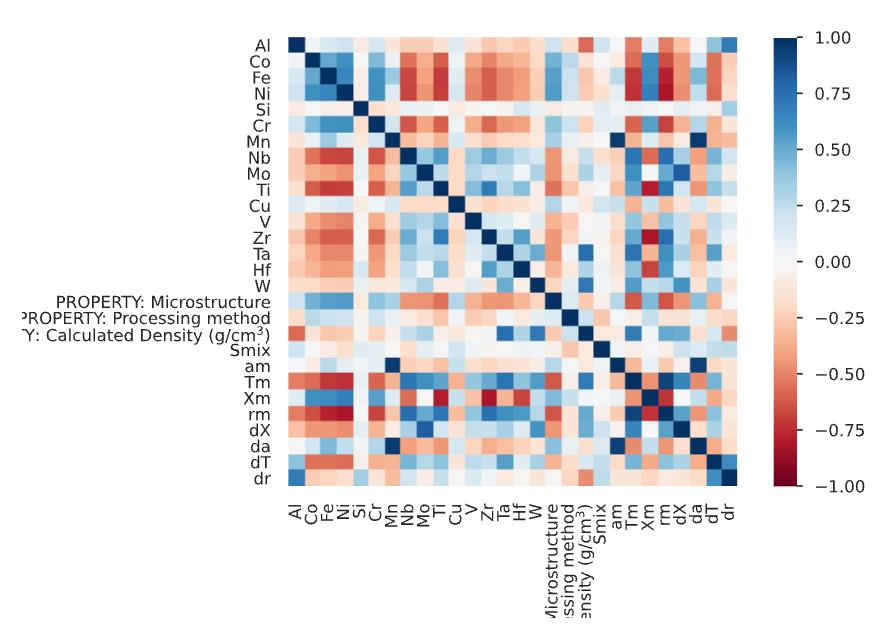
\includegraphics[height=8cm]{estrutura_dos_dados.jpg} 
    \caption{Correlação de Kendall's }
    \label{fig:kendals_correlacao_sem_duplicados}
\end{figure}
\FloatBarrier


\subsection{Normalização dos dados}\label{sec:MAT_MET_SEC_B_SUB_D}

Após remover os itens duplicados co conjunto de dados, foi verificado a redução da acurácia do modelo, que é justificado devido a algum tipo de overfitting do modelo, a ocorrência de dados duplicados são os principais responsáveis por ``viciar'' o modelo a determinado tipo de dado.

A próxima etapa será executada com o conjunto de dados sem os dados duplicados. Primeiramente precisamos subdividir as variáveis em normalizáveis e não normalizáveis. As variáveis normalizáveis são as que possuem alguma possibilidade de conter dados outliers, isto é, dados fora de um intervalo interquartil. Assim, os dados não normalizáveis foram os dados de composição química, uma vez que a composição química do conjunto de dados é definida por porcentagem, e o método de processamento, pois é uma variável categórica.

Os outros dados que são variáveis contínuas, passaram por um processo de normalização. 


\begin{table}[htb]
\centering
\caption{Conjunto de dados normalizados}
\begin{supertabular}{l|c|c|c|c}
\hline
{ microestruturas } & { precision } & { recall } & { f1-score } & { support }\\\hline
{ BCC } &           {0.692308} & {0.757009} & {0.723214} & {107.00000}\\\hline
{ BCC++ } &         {0.577778} & {0.393939} & {0.468468} & {66.00000}\\\hline
{ BCC B2 } &        {0.428571} & {0.580645} & {0.493151} & {31.00000}\\\hline
{ FCC } &           {0.513158} & {0.629032} & {0.565217} & {62.00000}\\\hline
{ FCC++ } &         {0.641026} & {0.471698} & {0.543478} & {53.00000}\\\hline
{ FCC BCC } &       {0.558140} & {0.571429} & {0.564706} & {42.00000}\\\hline
{ OTHER } &         {0.500000} & {0.476190} & {0.487805} & {21.00000}\\\hline
{ accuracy } &      {0.583770} & {0.583770} & {0.583770} & {0.58377}\\\hline
{ macro avg } &     {0.558711} & {0.554278} & {0.549434} & {382.00000}\\\hline
{ weighted avg } &  {0.589602} & {0.583770} & {0.579581} & {382.00000}\\\hline
\end{supertabular}
    \legend{}
    \label{table:relatorio_normalizados}
\end{table}


\begin{table}[htb]
\centering
\caption{Conjunto de dados com sobre amostragem}
\begin{supertabular}{l|c|c|c|c}
\hline
{ microestruturas } & { precision } & { recall } & { f1-score } & { support }\\\hline
{ BCC } &           {0.819444} & {0.797297} & {0.808219} & {74.000000}\\\hline
{ BCC++ } &         {0.783784} & {0.783784} & {0.783784} & {74.000000}\\\hline
{ BCC B2 } &        {0.835443} & {0.891892} & {0.862745} & {74.000000}\\\hline
{ FCC } &           {0.826087} & {0.770270} & {0.797203} & {74.000000}\\\hline
{ FCC++ } &         {0.794872} & {0.837838} & {0.815789} & {74.000000}\\\hline
{ FCC BCC } &       {0.847222} & {0.824324} & {0.835616} & {74.000000}\\\hline
{ OTHER } &         {0.905405} & {0.905405} & {0.905405} & {74.000000}\\\hline
{ accuracy } &      {0.830116} & {0.830116} & {0.830116} & {0.830116}\\\hline
{ macro avg } &     {0.830323} & {0.830116} & {0.829823} & {518.000000}\\\hline
{ weighted avg } &  {0.830323} & {0.830116} & {0.829823} & {518.000000}\\\hline
\end{supertabular}
    \legend{}
    \label{table:relatorio_oversampled}
\end{table}



\begin{table}[htb]
\centering
\caption{Conjunto de dados com sobre amostragem homologados}
\begin{supertabular}{l|c|c|c|c}
\hline
{ microestruturas } & { precision } & { recall } & { f1-score } & { support }\\\hline
{ BCC } &           {0.857143} & {0.909091} & {0.882353} & {33.000000}\\\hline
{ BCC++ } &         {1.000000} & {0.625000} & {0.769231} & {16.000000}\\\hline
{ BCC B2 } &        {0.700000} & {0.777778} & {0.736842} & {9.000000}\\\hline
{ FCC } &           {0.562500} & {0.500000} & {0.529412} & {18.000000}\\\hline
{ FCC++ } &         {0.818182} & {0.500000} & {0.620690} & {18.000000}\\\hline
{ FCC BCC } &       {0.541667} & {1.000000} & {0.702703} & {13.000000}\\\hline
{ OTHER } &         {0.666667} & {0.750000} & {0.705882} & {8.000000}\\\hline
{ accuracy } &      {0.730435} & {0.730435} & {0.730435} & {0.730435}\\\hline
{ macro avg } &     {0.735165} & {0.723124} & {0.706730} & {115.000000}\\\hline
{ weighted avg } &  {0.763591} & {0.730435} & {0.726443} & {115.000000}\\\hline
\end{supertabular}
    \legend{}
    \label{table:relatorio_oversampled_homolog}
\end{table}


Objetivos:
através de clusterização, o objetivo do trabalho proposto é a classificação de uma liga e a predição da tensão de escoamento e da fase presente na liga utilizando como parâmetro de entrada a composição química da liga e a sua densidade.

De início serão feitas diversas simulações com diferentes tipos de modelos cada um com sua particularidade. Com auxílio de indicadores estatísticos será decidida qual melhor ferramenta utilizar.

Primeiro passo será a análise exploratória dos dados, verificando quais tipos de dados presentes na base, ocorrência de campos ausentes ou com dados outliers.

Em seguida serão utilizados diferentes modelos disponíveis na biblioteca python scikit-learn e então compará-los com diferentes medidas estatísticas, matriz de confusão, acurácia, precisão. 

O conjunto de dados contem aproximadamente 600 amostras, com os seguintes parâmetros: nome das ligas, a composição química de cada elemento, e alguns dados empíricos como entropia de mistura, módulo de Young, microestrutura, densidade entre outros.


\section{Comparando Modelos}\label{sec:LABEL_CHP_5_SEC_A}

A biblioteca scikitlearn do python disponibiliza alguns modelos para treinar e classificar um conjunto de dados. Foram escolhidos 6 modelos para fazer essa comparação inicial. São eles GradientBoostingClassifier, RandomForestClassifier, MLPClassifier, KNeighborsClassifier, SVC e  DecisionTreeClassifier. 





Ao analisar o conjunto de dados, foi observado que os elementos químicos hora estão presentes pra algum grupos de ligas, e hora estão presentes em outros grupos. 
No primeiro treino e teste a acurácia apresentou resultados de aproximadamente 60\%, considerando um modelo geral para todo o conjunto de dados, porém o desvio padrão estava acima dos 10\%.

Após clusterizar os dados, foi gerado um modelo para cada grupo, e assim verificado a acurácia e o desvio padrão. Foram feitos agrupamentos para 3,5 e 7 clusters. 
os resultados estão na Tabela \ref{quad:clusters_acuracia}, utilizando o cross validation com 10 partiçções foram obtidos esses resultados:


\begin{table}[htb]
\centering
\caption{Clusters: 3 }
\begin{supertabular}{|c|c|c|c|c|}
\hline
{ cluster }&{ $\mu$(acurácia) }&{ $\sigma$(acurácia) }&{ qtde }&{ $(\%)$ }\\\hline
{ 1 } &
{ 0.785 } &
{ 0.123 } &
{ 135 } &
{ 28.7 }\\\hline
{ 2 } &
{ 0.704 } &
{ 0.081 }& 
{ 247 } &
{ 52.4 }\\\hline
{ 3 } &
{ 0.921 } &
{ 0.072 }&
{ 89 } &
{ 18.9 }\\\hline
\end{supertabular}
    \legend{}
    \label{quad:clusters_acuracia}
\end{table}





Variaveis experimentais importantes:
medir a resistencia mecanica - dizer a temeperatura

prever a fase - dizer como material foi sintetizado ( fundido, Tratamento térmico, fundição, sinterização .. ) 

\pagebreak


coeficiente de variacao 

https://www.cpt.com.br/artigos/em-estatistica-como-saber-se-um-desvio-padrao-e-grande-ou-pequeno

Atualmente temos para um conjunto de dados dividido em 10 partes uma acuracia media de $ 56\% $, e um desvio padrao de $ 9 \%$

O foco agora é encontrar um padrão de dados onde a acuracia e desvio padrao do modelo se comportem melhor, isto é, para alguns casos temos um pouco de overfiting no modelo, ocasionando discrepancias na previsao quando a liga possui uma gama de elementos que de certa forma é um outlier para o conjunto geral dos dados.









\section{Tratamento dos dados}\label{sec:MAT_MET_SEC_C}

Para o conjunto de dados utilizado, não será avaliado o tipo de teste (tração/compressão) nem a tensão de escoamento, sendo assim, essas colunas foram removidas do conjunto de dados.

Além disso, após remover essas colunas foi feita uma limpeza de linhas duplicadas, sendo assim de um total de 589 dados, sobraram 382. Isso permitiu que o desvio padrão do treinamento do modelo fosse reduzido, uma vez que com dados repetidos, estava ocasionando overfitting no modelo.



\clearpage
\section{Exemplos de Citações}
{\centering\bfseries\color{red}
Exemplos de Citações
\par}

{\centering\bfseries\color{red}
Citação direta:
\par}

\bigskip

Citações diretas de até 3 linhas, devem iniciar e terminar por aspas duplas.\\

Se o texto original já contiver aspas duplas, substituí-las por aspas simples. A indicação da fonte da citação pode
estar inserida no texto ou após a citação.\\

\bigskip

{\color{red}
Exemplo:}

\bigskip

Segundo Castro (2001, p. 23): {\textquotedbl}Os deveres da conduta do anestesiologista constituem predicados importantes
quando se quer avaliar a qualidade do procedimento.{\textquotedbl}\\

\bigskip

{\color{red}
ou}

\bigskip

{
{\textquotedbl}A expressão 'furiosa' dessa estátua de que fala Rebelais, corresponde também à realidade.{\textquotedbl}
(BAKHTIN, 1987, p. 89).}

\bigskip

{\centering\bfseries\color{red}
Citação Direta com mais de três linhas:
\par}

\bigskip

As citações diretas, no texto, com mais de três linhas, devem ser
destacadas com recuo de 4 cm da margem esquerda, com letra menor que a do texto utilizado e sem as aspas. A indicação da fonte da citação pode estar inserida no texto ou após a citação. \\ 

\bigskip

{\color{red}
Exemplo:}
\bigskip
Sobre mercado financeiro, Fortuna (1996, p. 15) considera:\\
\bigskip

\begin{citacao}
O mercado financeiro permite que um agente econômico qualquer, sem perspectivas de aplicação, em algum empreendimento
próprio, da poupança que é capaz de gerar, seja colocado em contato com outro, cujas perspectivas de investimento
superam as respectivas disponibilidades de poupança.\\
\end{citacao}

\bigskip
A seguir uma citação em inglês:\\

\begin{citacao}[english]
This text is an example in English language in italic with correct hyphenation. This text is an example in English language in italic with correct hyphenation. This text is an example in English language in italic with correct hyphenation.
\end{citacao}
\bigskip

\clearpage{\centering\bfseries\color{red}
Citação Indireta:
\par}

\bigskip

Não se utilizam aspas para esse tipo de citação, nem a(s) página(s) de onde foi extraída a ideia.\\

\bigskip

{\color{red}
Exemplo:}

\bigskip
esse aqui 

A bíblia começou a ser escrita no ano 1.000 a.C. e foi finalizada em 100 d.C., com a morte do último apóstolo, São João, levando aproximadamente 1.150 anos para ser concluída \cite{book:GHELLER}.\\


\bigskip

{\centering\bfseries\color{red}
Citação de Citação:
\par}

\bigskip

A indicação da fonte é feita pelo sobrenome do autor da obra citada (não consultada), ano, seguido da expressão latina apud. Após, indica-se o sobrenome do autor da obra consultada, seguido do ano de publicação, precedido por vírgula. Quando for citação direta incluir a(s) página(s) após a data de publicação, precedida de vírgula.\\

\bigskip

{\sffamily
\textrm{\textcolor{red}{Exemplo no texto}}\textrm{:}}

\bigskip

{\sffamily
\textrm{citado por }}

\bigskip

{\sffamily
\textrm{Segundo Marques e Ribeiro}\footnote{\ MARQUES, Alberto; RIBEIRO, \textbf{Angela. As fazendas agrícolas}. São
Paulo: Ática, 2000. 350 p.}\textrm{ (2000 }\textrm{\textcolor{black}{apud }}\textrm{OLIVEIRA, 2001), \apudonline {art:PRADO}{book:AMADO} o Serviço de
Atenção Médico-Sanitário da Suécia tem uma tradição de mais de cem anos. }}

\bigskip

{\color{red}
ou}

{\sffamily
\textrm{\textcolor{red}{Em nota de rodapé}}\textrm{:}}

\bigskip

{\centering\bfseries\color{red}
Indicação da Citação:
\par}

\bigskip

{\sffamily
\textrm{Se a indicação da fonte da citação estiver incluída na frase, a mesma deve aparecer apenas com a inicial
maiúscula seguida de parênteses, com a data de publicação do }\textrm{documento. Quando for citação direta incluir a(s)
página(s) após a data de publicação, precedida de vírgula.}}

\bigskip

{\color{red}
Exemplo com autor pessoal:}

\bigskip

Segundo Fonseca(2004, p. 36): {\textquotedbl}Se não houver mecanismos jurídicos que assegurem a proteção dos direitos
humanos, esse valor não será concretizado pelo Poder Público.{\textquotedbl}\\

\bigskip

{\sffamily
\textrm{\textcolor{red}{Exemplo com dois autores: }}}

\bigskip

Tonetto e Reck (2001, p. 134) destacam: {\textquotedbl}Este autoconhecimento pressupõe conhecer seus limites
[...]{\textquotedbl} \\

\bigskip

{\color{red}
Exemplo com mais de três autores:}

\bigskip

Neste contexto, Couto e outros (2004, p. 52) destacam que: {\textquotedbl}No capitalismo não é a simples ausência do
patrão que promove a superação do despotismo da divisão laboral.{\textquotedbl}\\

\bigskip

{\sffamily
\textrm{\textcolor{red}{Exemplo com autor institucional: }}}

\bigskip

De acordo com a Pontifícia Universidade Católica do Rio Grande do Sul (2001, p. 24): {\textquotedbl}[...] no horizonte 2001/2010, o esforço estratégico da PUCRS será centrado em sete áreas estratégicas [...]{\textquotedbl}\\

\bigskip

{\color{red}
Exemplo sem autor(es), com a entrada pelo título:}

\bigskip

Segundo o Guia de clareamento dental (1996, p. 8): {\textquotedbl}A causa mais comum do escurecimento dental é o tratamento endodôntico realizado de modo inadequado e sem os cuidados técnicos.{\textquotedbl}\\

\bigskip

{\color{red}
Exemplo sem autor(es), com a entrada pelo título que inicia por artigo:}

\bigskip

O movimento social, com o intuito de realizar uma transformação social, é uma das tarefas mais importantes da atualidade
(O COOPERATIVISMO..., 2002).\\

\bigskip

As citações a seguir foram colocadas para que as referências aparecessem na bibliografia. Como exemplo temos os livro de Jorge Amado \cite{book:AMADO}  \cite{book:AMADO2}, e este autor que desconheço \cite{book:OHANSSON}, além de \cite{book:ENGEL} e um artigo \cite{art:PRADO}. Notem que é gerado um link hipertexto no documento em PDF.


\chapter{CONCLUSÃO}

O desenvolvimento de novas ligas de Alta Entropia podem oferecer diversas opções com propriedades tão boas quanto, ou até melhores, que ligas convencionais comuns. Como essas ligas são ainda um tema considerado recente na linha de pesquisa e desenvolvimento, as informações sobre essas ligas são limitadas. Sendo assim, para uma possível redução de custos na sua fase inicial de desenvolvimento, uma excelente alternativa é o uso de inteligência artificial utilizando os conjuntos de dados disponíveis na literatura, para obter uma previsão de que tipo de microestrutura será esperada para uma faixa de composição química arbitrária. 

No presente estudo, foi verificado que com uma limitada quantidade de amostras de 382 dados, podemos obter uma acurácia de um pouco mais de 80\% utilizado os dados rebalanceados com a sobreamostragem, e uma acurácia de quase 60\% utilizando 30\% dos dados separados para teste. Um modelo de aprendizado de máquina pode ser aplicado em diversas categorias, seja para área da saúde, legislação, mercado financeiro, entre outros. No caso deste trabalho, o uso de inteligência artificial, contribuiu para prever a microestrutura de ligas de alta entropia, utilizando a sua composição química em porcentagem, os valores de entropia de mistura, constante de rede, temperatura de fusão, entre outras características citadas nos materiais e métodos.


Em projetos de aprendizado de máquina mais evoluídos, o conjunto de dados costuma estar na casa de milhares. E no caso deste estudo com aproximadamente 400 dados, podemos obter uma classificação satisfatória de ligas de alta entropia. Assim, para os estudos futuros, conforme  maior disponibilidade dos dados, o uso de inteligência artificial poderá ser um forte aliado para redução de custos em pesquisas e desenvolvimento de novas ligas. O compartilhamento e a cooperatividade entre diferentes centros de pesquisas é o fator fundamental para evoluir a linha de pesquisa acadêmica em sinergia com uso de ferramentas de aprendizado de máquina, pois o uso desses algoritmos permitem que a comunidade acadêmica desenvolva novas ligas com mais assertividade a partir de simulações, e caso necessário corrigir o modelo conforme necessário. 



% Onde se expõe o fechamento das ideias do estudo, são apresentados os resultados da pesquisa, e partindo da análise destes resultados, tiram-se as conclusões e se for necessário, as sugestões relativas ao estudo. \\

% Observação: É opcional a apresentação dos desdobramentos relativos à importância, síntese, projeção, repercussão, encaminhamento e outros.

\postextual
%%%%%%%%%%%%%%%%%%%%%%%%%%%%%%%%%%%%%%%%%%%%%%%%%%%%
% R E F E R Ê N C I A S  (OBRIGATÓRIO)
%%%%%%%%%%%%%%%%%%%%%%%%%%%%%%%%%%%%%%%%%%%%%%%%%%%%

\bibliography{elementos-postextuais/referencias.bib}

%%%%%%%%%%%%%%%%%%%%%%%%%%%%%%%%%%%%%%%%%%%%%%%%%%%%
% G L O S S A R I O (opcional)
%%%%%%%%%%%%%%%%%%%%%%%%%%%%%%%%%%%%%%%%%%%%%%%%%%%%
\clearpage
\addcontentsline{toc}{chapter}{GLOSSÁRIO} %\glossaryname
\printglossary

%%%%%%%%%%%%%%%%%%%%%%%%%%%%%%%%%%%%%%%%%%%%%%%%%%%%%%%%%
% A P Ê N D I C E S  (Opcional) 
%%%%%%%%%%%%%%%%%%%%%%%%%%%%%%%%%%%%%%%%%%%%%%%%%%%%%%%%%
%\textrm{\textcolor{red}{Apêndice(s) (Este item é elaborado 
% pelo próprio autor do trabalho e serve para  complementar
% a sua argumentação.  É um elemento \textbf{opcional)}.}}
%%%%%%%%%%%%%%%%%%%%%%%%%%%%%%%%%%%%%%%%%%%%%%%%%%%%%%%%

\clearpage
\begin{apendicesenv}

\begin{vplace}
{\centering
\ABNTEXchapterfont{\textrm{APÊNDICES}}
\par}
\end{vplace}
\newpage
{\let\clearpage\relax \chapter{\textnormal{Análise dos
relatórios mensais de uso do serviço de renovação de empréstimos.}}}

Lorem ipsum dolor sit amet, consectetur adipiscing elit. Donec lacus nisl, ultricies vitae semper eu, scelerisque nec enim. Curabitur posuere tortor orci, at porta leo laoreet et. Quisque ut congue dolor. Maecenas vel sagittis diam. Praesent fermentum eleifend mi, sit amet vehicula leo pellentesque quis. Curabitur mattis luctus pulvinar. Proin auctor est nec nulla pellentesque commodo. Donec nec justo eu magna aliquet eleifend. Curabitur tristique tortor id sem dignissim, a iaculis metus interdum. Phasellus bibendum velit sit amet interdum semper. Nam vestibulum dui quis nisi consectetur, id vehicula dolor faucibus.\\
\newpage
{\let\clearpage\relax \chapter{\textnormal{Análise dos
relatórios mensais de uso do serviço de empréstimo domiciliar.}}}

Lorem ipsum dolor sit amet, consectetur adipiscing elit. Donec lacus nisl, ultricies vitae semper eu, scelerisque nec enim. Curabitur posuere tortor orci, at porta leo laoreet et. Quisque ut congue dolor. Maecenas vel sagittis diam. Praesent fermentum eleifend mi, sit amet vehicula leo pellentesque quis. Curabitur mattis luctus pulvinar. Proin auctor est nec nulla pellentesque commodo. Donec nec justo eu magna aliquet eleifend. Curabitur tristique tortor id sem dignissim, a iaculis metus interdum. Phasellus bibendum velit sit amet interdum semper. Nam vestibulum dui quis nisi consectetur, id vehicula dolor faucibus.\\
\end{apendicesenv}

%%%%%%%%%%%%%%%%%%%%%%%%%%%%%%%%%%%%%%%%%%%%%%%%%%%%%%%%%
% A N E X O S   (Opcional) 
%%%%%%%%%%%%%%%%%%%%%%%%%%%%%%%%%%%%%%%%%%%%%%%%%%%%%%%%%
% \textrm{\textcolor{red}{Anexos (Este item é constituído por 
% documentos complementares ao texto do trabalho e que não são 
% elaborados pelo autor do mesmo, servem para fundamentação, 
% comprovação e ilustração. É um elemento \textbf{opcional}).}}
%%%%%%%%%%%%%%%%%%%%%%%%%%%%%%%%%%%%%%%%%%%%%%%%%%%%%%%%%

\clearpage
\begin{anexosenv}

\begin{vplace}
{\centering
\ABNTEXchapterfont{ANEXOS}
\par}
\end{vplace}
\newpage
{\let\clearpage\relax \chapter{\textnormal{Demonstrativo de
frequência diária ago./set. 2001}}}

Lorem ipsum dolor sit amet, consectetur adipiscing elit. Donec lacus nisl, ultricies vitae semper eu, scelerisque nec enim. Curabitur posuere tortor orci, at porta leo laoreet et. Quisque ut congue dolor. Maecenas vel sagittis diam. Praesent fermentum eleifend mi, sit amet vehicula leo pellentesque quis. Curabitur mattis luctus pulvinar. Proin auctor est nec nulla pellentesque commodo. Donec nec justo eu magna aliquet eleifend. Curabitur tristique tortor id sem dignissim, a iaculis metus interdum. Phasellus bibendum velit sit amet interdum semper. Nam vestibulum dui quis nisi consectetur, id vehicula dolor faucibus.\\
\newpage
{\let\clearpage\relax \chapter{\textnormal{Demonstrativo de frequência diária jan./dez. 2002}}}

Lorem ipsum dolor sit amet, consectetur adipiscing elit. Donec lacus nisl, ultricies vitae semper eu, scelerisque nec enim. Curabitur posuere tortor orci, at porta leo laoreet et. Quisque ut congue dolor. Maecenas vel sagittis diam. Praesent fermentum eleifend mi, sit amet vehicula leo pellentesque quis. Curabitur mattis luctus pulvinar. Proin auctor est nec nulla pellentesque commodo. Donec nec justo eu magna aliquet eleifend. Curabitur tristique tortor id sem dignissim, a iaculis metus interdum. Phasellus bibendum velit sit amet interdum semper. Nam vestibulum dui quis nisi consectetur, id vehicula dolor faucibus. \\

\end{anexosenv}

%%%%%%%%%%%%%%%%%%%%%%%%%%%%%%%%%%%%%%%%%%%%%%%%%%%%%%%%%
% F I M   D O  D O C U M E N T O
%%%%%%%%%%%%%%%%%%%%%%%%%%%%%%%%%%%%%%%%%%%%%%%%%%%%%%%%%
\end{document}